\documentclass[font=plain]{abnt}
\usepackage[utf8]{inputenc}
\usepackage[brazil]{babel}
\usepackage[title, abnt-etal-cite=3]{abntcite}
\usepackage{graphicx}
\usepackage{graphicx,color} 
\usepackage{placeins} % para posicionamento das imagens
\usepackage{paralist}
\usepackage{subfloat} 
\usepackage{subfig} 
\usepackage{multirow}
\usepackage{lscape}
\usepackage{scalefnt}
\usepackage{algpseudocode,algorithm}
\usepackage{amsmath,amsfonts}   % \mathbb, para fontes matematicas
\usepackage{amssymb,amsthm}  
\usepackage{verbatim}
% Declaracoes em Português
\algrenewcommand\algorithmicend{\textbf{fim}}
\algrenewcommand\algorithmicdo{\textbf{faça}}
\algrenewcommand\algorithmicwhile{\textbf{enquanto}}
\algrenewcommand\algorithmicfor{\textbf{para}}
\algrenewcommand\algorithmicif{\textbf{se}}
\algrenewcommand\algorithmicthen{\textbf{então}}
\algrenewcommand\algorithmicelse{\textbf{senão}}
\algrenewcommand\algorithmicreturn{\textbf{devolve}}
\algrenewcommand\algorithmicfunction{\textbf{função}}

% Rearranja os finais de cada estrutura
\algrenewtext{EndWhile}{\algorithmicend\ \algorithmicwhile}
\algrenewtext{EndFor}{\algorithmicend\ \algorithmicfor}
\algrenewtext{EndIf}{\algorithmicend\ \algorithmicif}
\algrenewtext{EndFunction}{\algorithmicend\ \algorithmicfunction}

% O comando For, a seguir, retorna 'para #1 -- #2 até #3 faça'
\algnewcommand\algorithmicto{\textbf{até}}
\algrenewtext{For}[3]%
{\algorithmicfor\ #1 $\gets$ #2 \algorithmicto\ #3 \algorithmicdo}

\instituicao{UNEB - Universidade do Estado da Bahia 
             \par Departamento de Ciências Exatas e da Terra}
\titulo{ \sf\textbf{Planejamento e mapeamento de trajetórias em tempo real para navegação de robôs humanóides em ambiente simulado 3D}}
\autor{Alan dos Santos Soares}
\orientador{Marco Antonio Costa Simões}
\coorientador{Diego Gervasio Frías Suárez}

\comentario{Trabalho de Conclusão de Curso apresentado a Universidade do Estado da Bahia como requisito parcial para obtenção do título de Bacharel em Sistemas de Informação.}
\local{Rua Silveira Martins, 2555, Cabula, Salvador-BA}
%esta data deve ficar estática após entrega final
\data{\today}

\begin{document}
    \DeclareGraphicsExtensions{.jpg,.pdf,.mps,.png,.bmp,.eps}
    
    % CAPA DA MONOGRAFIA 
    \begin{center}
      
      %\capa % geracao de capa automatica
	
	\begin{figure}[H]
	    \centering
	    
\includegraphics[scale=0.3]{figuras/logouneb.png}
	\end{figure}

      %\vspace*{\fill}
      
      	\begin{center}
	 %\ABNTchapterfont
	 %\bfseries
	 \sf{Universidade do Estado da Bahia \\}
	 \sf{Departamento de Ci\^encias Exatas e da Terra \\}
	 \sf{Bacharelado em Sistemas de Informação \\}
	\end{center}
      	
	\vspace*{3 cm}

	\begin{center}
	 %\ABNTchapterfont
	 %\bfseries
	 \sf\Large\textbf{Planejamento e mapeamento de trajetórias em tempo real para navegação de robôs humanóides em ambiente simulado 3D}
	\end{center}
	
	\vspace*{3 cm}

	{\large \textbf{Alan dos Santos Soares}}

	\begin{center}
	\vspace*{\fill}
	%\vspace*{0.5cm}
	Rua Silveira Martins, 2555, Cabula, Salvador-BA
	\par
	13 de Julho de 2014
	\vspace*{1cm}
	\end{center}
      
    \end{center}
    
    % CONTRA CAPA DA MONOGRAFIA     
    \folhaderosto % geracao de folha de rosto automatica

    %Folha de Aprovação
    \begin{folhadeaprovacao}
    
	\begin{center}

	{\large \textbf{Alan dos Santos Soares}}
	
	\vspace*{\fill}\vspace*{\fill}
	
	\begin{center}
	 %\ABNTchapterfont
	 %\bfseries
	 \sf\Large\textbf{Planejamento e mapeamento de trajetórias em tempo real para navegação de robôs humanóides em ambiente simulado 3D}
	\end{center}

	\vspace*{\fill}
	
	\hspace{.45\textwidth}
	\begin{minipage}{.5\textwidth}
	Trabalho de Conclusão de Curso apresentado a Universidade do Estado da Bahia como requisito parcial para obtenção do título de Bacharel em Sistemas de Informação.
	\end{minipage}
	
	\end{center}
	
	Data de aprovação :
	\setlength{\ABNTsignthickness}{0.4pt}
	\setlength{\ABNTsignskip}{2cm}
	\hspace*{1cm}
	\assinatura{Prof. Marco Antonio Costa Simões\\MSc. em Ciência da Computação\\ Universidade do Estado da Bahia}
	\assinatura{Prof. Diego Gervasio Frías Suárez\\PhD. em Modelagem Computacional\\ Universidade do Estado da Bahia}
	\assinatura{Prof. Josemar Rodrigues de Souza\\PhD. em Informática\\ Universidade do Estado da Bahia}
	
	\begin{center}
	\vspace*{\fill}
	%\vspace*{0.5cm}
	Rua Silveira Martins, 2555, Cabula, Salvador-BA
	\par
	13 de Junho de 2014
	\vspace*{1cm}
	\end{center}
	
	
	
    \end{folhadeaprovacao}
    
    %%%%%%%%%%%%%%%%%%%%%%%%%%%%%%%%%%%%%%%%%%%%%%%%%%%%%%%%%%%%%%%%%%%%%%%%%%%%%%%
%% Este arquivo faz parte do template de TCC baseado nas normas da ABNT 
%%  voltado para alunos da UEFS
%% Desenvolvimento: Danilo de Oliveira Gonçalves
%% Adaptação final: João Carlos Nunes Bittencourt
%% Data: 31/03/2011
%%%%%%%%%%%%%%%%%%%%%%%%%%%%%%%%%%%%%%%%%%%%%%%%%%%%%%%%%%%%%%%%%%%%%%%%%%%%%%%


% dedicatória (opcional)
%\begin{dedicatoria}
%Ainda vou fazer.
%\end{dedicatoria}

\vfill

\begin{flushright}
\hfill \textit{Dedico esta monografia a minha família,\\pelo apoio fornecido e aos meus amigos.\\}
\end{flushright}

\vspace*{1cm}

\clearpage 

    
\begin{center}
 	{\large \textbf{Agradecimentos}}
\end{center}

Agradeço primeiramente a minha mãe Alaide Cruz dos Santos Soares que me ensinou e me educou 
durante toda a minha vida, me dando apoio e amparo nos momentos bons e ruíns quando eu mais 
precisei.  

Aos meus professores e orientadores Diego Gervásio Frias Suárez e Marco Antonio Costa Simões 
pelos sábios ensinamentos, críticas, pelas experi\^encias compartilhadas e pela atenção dada 
nos momentos em que eu mais precisei.

A todos os meus familiares, irmão e irmãs que contribuiram direta e indiretamente para que eu pudesse chegar ao final do curso, em especial a minha tia Clarice Santos, que sem ela eu não teria conseguido 
efetuar a minha matricula no curso.

A todos os meus colegas de faculdade, em especial a Leandreson Ferreira e Leone de Jesus por 
toda a experi\^encia vivida durante o período acad\^emico.

E por fim, a todos os membros do grupo de pesquisa ACSO/BRT/UNEB, pelas experi\^encias compartilhadas, pelas risadas descontraídas, pelo conhecimento compartilhado e por tudo que conquistei estando presente em um dos melhores grupos de pesquisa da Bahia/Brasil.
    \begin{resumo}
%Escrever um texto que contemple todo o conteúdo do trabalho, com espaçamento
%1,5, justificado. Conforme as normas NBR 14724:2011 e NBR 6028:2003,da ABNT,
%o resumo é elemento obrigatório, constituído de parágrafo único; uma seqüência de
%frases concisas e objetivas e não de uma simples enumeração de tópicos, não
%ultrapassando 500 palavras, O resumo deve ressaltar o objetivo, o método, os
%resultados e as conclusões do documento. Deve-se usar o verbo na voz ativa e na
%terceira pessoa do singular. Devem ser seguido, logo abaixo, das palavras
%representativas do conteúdo do trabalho, isto é, palavras-chave e/ou descritores,
%que são palavras principais do texto, sendo de 3 a 5, separadas por ponto)

A necessidade da automatização e da construção de agentes robóticos capazes de realizar tarefas complexas, perigosas, 
delicadas, em ambientes din\^amicos, tornou-se um desafio aos investigadores. Alguns desses desafios incluem o mapeamento 
de ambientes din\^amicos, planejamento de trajetória e a predição de colisão. Este trabalho propõe um modelo 
para mapeamento e planejamento de trajetórias com predição de colisão para agentes robóticos em ambiente simulado. O modelo 
foi desenvolvido utilizando o time base do BahiaRT, desenvolvido pelo grupo de pesquisa ACSO/UNEB em parceria com o 
FCPortugal(FEUP-LIACC/Univ. Aveiro). A validação do projeto foi realizada utilizando uma aplicação de passe em futebol 
robótico integrado ao modelo proposto.

\textbf{Palavras-chaves}: Mapeamento. Planejamento de trajetórias. Predição. Simula\c{c}\~ao 3D.
\end{resumo}	

    \begin{abstract}
The need for automation and construction of robotic agents capable of performing complex tasks, 
dangerous, delicate in dynamic environments, it has become a challenge for researchers. Some of 
these challenges include mapping of dynamic environments, path planning and collision prediction. 
This work proposes a model for mapping and path planning with collision prediction for 
robotic agents in a simulated environment. The model was developed using the BahiaRT team base, 
developed by the research group ACSO / UNEB in partnership with FCPortugal (FEUP-LIACC/Univ. Aveiro). 
The validation of the project was performed using an application of the pass in robotic soccer 
integrated in the proposed model.

\textbf{Key-words}: Mapping. Path planning. Navigation. Prediction. Simulation 3D.
\end{abstract}


    \listadefiguras % geracao automatica da lista de figuras
    \listadetabelas % geracao automatica da lista de tabelas
    
    \pretextualchapter{Lista de abreviaturas e siglas}
    \begin{description}
      \item[ACSO]{Núcleo de Arquitetura de Computadores e Sistemas Operacionais}
      \item[DARPA]{Defense Advanced Research Projects Agency}
      \item[IA]{Inteligencia Artificial}
      \item[IAD]{Inteligencia Artificial Distribuida}
      \item[OBR]{Olimpíada Brasileira de Robótica}
      \item[PEAS]{Performance Environment Actuators Sensors}
      \item[SMA]{Sistemas Multi-Agente}
      \item[TDP]{Team Description Paper}
    \end{description}
    
 %   \pretextualchapter{Lista de símbolos}
 %   \begin{description}
 %     \item[$ \pi $] Letra grega pi
 %     \item[$ \Pi $] Letra grega pi
 %   \end{description}
    
    \pretextualchapter{Lista de algoritmos}
    \begin{description}
      \item[$ 3.1 $] Implementação da verificação da presença de obstáculos . . . . . . . . . . . . .  p.35
      \item[$ 3.2 $] Implementação da predição de colisão . . . . . . . . . . . . . . . . . . . . . . . .  p.41
    \end{description}
    
    \sumario
    %---------- Primeiro Capitulo ----------
\chapter{Introdu\c{c}\~ao}
%Faça a justificativa desse tema. Por quais motivos essa pesquisa é relevante e importante? Apresente argumentos que justificam a importância da pesquisa no âmbito do seu campo de conhecimento e a relevância social do estudo (motivos e relevância da escolha do tema, levando em conta formação pessoal e pertinência/ contribuição acadêmica).
Um dos principais desafios no campo da robótica, é a forma como os agentes humanóides buscam uma trajetória para chegar a 
um determinado objetivo. No ambiente em que o agente está atuando existem diversos obstáculos que podem comprometer 
a sua locomoção no ambiente, principalmente se os obstáculos não forem estáticos.

Assim como o futebol de robôs, o desenvolvimento de veículos autônomos, designado como qualquer veículo com capacidade de
transporte de pessoas ou bens sem a utilização de um condutor humano, é um dos desafios que requerem o planejamento e mapeamento de 
trajetórias em tempo real para evitar colisão com obstáculos móveis da mesma forma que o futebol de robôs.

A construção de veículos terrestres
autônomos tem como principais objetivos, reduzir os acidentes de trânsito provocados por fatores humanos, aumentar a produtividade 
e otimizar os recursos veiculares através da utilização adequada de componentes. Para fomentar e estimular pesquisas no 
desenvolvimento de veículos autônomos, desafios como o DARPA Urban Challenge e o DARPA Grand Challenge foram criados \cite{darpa}.

Outro desafio hoje em destaque é o desenvolvimento de robôs de serviço. Estes são robôs autônomos capazes de se mover em um ambiente 
dinâmico para realizar tarefas úteis para o bem estar de humanos e a preservação de equipamentos físicos, necessitando planejar uma 
trajetória de forma eficiente e segura, evitando causar acidentes. Segundo \citeonline{dudek} e \citeonline{siegwart}, o estudo das
questões computacionais envolvidas na movimentação não supervisionada de robôs é fundamental para se obter sucesso no 
desenvolvimento de agentes capazes de atuarem em ambientes dinâmico e contínuo.

%O principal problema dos planejadores de trajetórias atuais, é que foram desenvolvidos para ambientes estáticos\cite{}, o que implica no
%não funcionamento quando este é utilizado em um ambiente dinâmico e contínuo, onde o resultado das ações não é determinístico. A partir 
%dessa lacuna, o estudo sobre a predição de estados do ambiente e dos obstáculos em sua volta em função de suas
%ações realizadas e da análise do comportamento dos obstáculos permite uma maior mobilidade do agente.

Para fomentar a investigação, uma organização internacional chamada RoboCup \cite{robocup} foi formada. O objetivo é promover e estimular 
pesquisas nas áreas de Inteligência Artificial Distribuída (IAD) e Robótica Inteligente, colocando problemas de investigação distintos 
, mas ao mesmo tempo interrelacionados.

A sub-liga da RoboCup, Simulação 3D \cite{SimulationLeague}, primeira dentre as simuladas a representar um robô humanóide em sua 
competição, tem como desafio padrão o futebol de robôs, dispondo de um vasto conjunto de desafios aos investigadores. Tais desafios 
como  desenvolvimento do controle de baixo nível de robôs humanóides e a criação de comportamentos básicos e eficiêntes como levantar 
e correr são essenciais para se ter um time competitivo. Algumas das características do domínio e desafios associados mais 
importantes colocados pelo simulador incluem simulação em tempo real, modelo energético realista, comunicação pouco confiável e 
com baixa largura de banda, percepção e ações assíncronas, ambiente multi-objetivo, parcialmente cooperativo e parcialmente 
adverso \cite{bReis2001}. O futebol de robôs configura-se, portanto, como uma plataforma universal 
para testes avançados em robótica autônoma com possibilidades em aplicações em diversas áreas.

%Objetivo
Este trabalho tem como objetivo propor e validar um modelo de mapeamento e planejamento de trajetórias de agentes humanóides no
ambiente simulado 3D no contexto de jogo de futebol de robôs utilizando o time base BahiaRT do grupo de pesquisa 
ACSO (Nucleo de Arquitetura de Computadores e Sistemas Operacionais) da UNEB. O time possui uma parceria com 
time FCPortugal (FEUP-LIACC / Univ. Aveiro) de agentes simulados 3D, que tem como objetivo construir agentes 
totalmente autônomos e inteligentes e vencer a sub-liga 3D da RoboCup.

Para validar o modelo proposto, uma aplicação de passe foi desenvolvida. Este tem como objetivo ser utilizado para gerar situações 
estratégicas que aumentem a chance de uma jogada bem sucedida. Porém, o sucesso de um passe depende não somente da escolha da melhor
trajetória da bola, mais também da predição de interceptação da bola e de comportamentos básicos eficientes como se posicionar e 
chutar a bola.

O estudo e desenvolvimento do projeto na área de robôs humanóides simulados, atende à necessidade estratégica
de continuar criando competências e desenvolvendo {\it know-how} próprio no estado da Bahia e no país na área de robótica autônoma. Este 
contribui para não sermos, em um futuro imediato, meros consumidores de tecnologia desenvolvida em outros estados e outros países.

Este trabalho está dividido em 5 capítulos. O Capítulo 2 se refere aos conceitos teóricos do problema e uma descrição do futebol 
de robôs.

No Capítulo 3 são descritos os trabalhos correlatos, o objetivo do trabalho, a metodologia utilizada e o modelo desenvolvido.

No Capítulo 4 é apresentada a descrição da metodologia de teste utilizada, a arquitetura do ambiente de teste, as métricas utilizadas 
para avaliar o modelo e os resultados obtidos.

Por último, o Capítulo 5 descreve as considerações finais e os trabalhos futuros.

    %\chapter{Fundamentos de Futebol de Robôs, Sistemas Multi-Agente e Planejamento de Trajetória}
\chapter{Fundamentos de robótica e planejamento de trajetória}
\label{chap:fundam}
O objetivo deste capítulo é fazer uma contextualização do modelo desenvolvido descrevendo as principais abordagens 
de Sistemas Multi-Agente (SMA), seus principais benefícios, tanto dentro como fora da área da robótica. Neste capítulo também 
é feito uma elucidação do conceito de planejamento de trajetória e alguns trabalhos relacionados. Além disso, 
é feita uma descrição de plataformas utilizadas no desenvolvimento de pesquisa na área de robótica no contexto de futebol 
de robôs em ambiente simulado.

Na Seção \ref{sec:sma} é feita uma descrição do conceito de SMA e os principais benefícios de sua 
utilização. São também introduzidos conceitos de comunicação em SMA na sub Seção \ref{subsec:comsma}. 
Por fim, na sub Seção \ref{subsec:coosma} são descritos os tipos de coordenação em SMA e o tipo de 
coordenação utilizada no BahiaRT para alcançar o objetivo deste projeto.

A Seção \ref{sec:futebolderobos} tem como objetivo realizar uma contextualização do objetivo deste trabalho. Na sub Seção
\ref{subsec:ligasdarobocup} é feita uma breve descriçao da RoboCup e algumas ligas padrões definidas como desafios. Na 
sub Seção \ref{subsec:xadrezvsrobocup} é realizada uma abordagem do Xadrez computacional e do futebol de robôs. Nas sub Seçôes 
\ref{subsec:roboviz}, \ref{subsec:simspark} são descritas as plataformas utilizadas na simulação 3D que é descrita na sub Seção 
\ref{subsec:simulacao3d} e posteriormente descrito os principais times campeões dos últimos anos na RoboCup na liga de simulação 3D 
na sub Seção \ref{subsec:times3d}.

Por último, a Seção \ref{sec:planejamentodetrajetorias} descreve o conceito de planejamento de trajetória, alguns trabalhos 
relacionados e os desafios em aberto.

\section{Sistemas Multi-Agente (SMA)}
\label{sec:sma}
Um SMA é um sistema composto por múltiplos agentes interagindo em um ambiente compartilhado. Cada agente
tem a capacidade de agir de forma autônoma tomando decisões que o levarão a atingir o seu objetivo. A interação entre os agentes 
pode ser realizada através de protocolos que são baseados em comportamentos humano. Tal interação tem como objetivo realizar a 
coordenação, cooperação, competição ou negociação dos agentes \cite{reisTese}.

Os SMA tem como objetivo resolver um problema de forma distribuída, aumentando a eficiência da resolução de um problema. Existem 
diversos fatores que demonstram que a utilização de SMA podem trazer benefícios para resolver determinados problemas \cite{stone}:

\begin{enumerate}
 \item O paralelismo, atribuindo diferentes tarefas a diferentes agentes de forma que sua execução seja mais rápida;
 \item A robustez, pois utilizam-se diferentes agentes, não existindo desta forma um ponto único de falha no sistema;
 \item A escalabilidade, permitindo o aumento de agentes de um determinado sistema aberto;
 \item A simplificação das tarefas individuais, dividindo o problema global em subproblemas;
 \item A manutenção da privacidade da informação e conhecimentos individuais de cada agente.
\end{enumerate}

Na Inteligência Artificial (IA), a utilização de SMA trazem diversos benefícios, principalmente da rentabilidade de recursos para 
problemas onde o conhecimento ou atividade é distribuída:

\begin{enumerate}
 \item Resolução mais rápida de problemas por conta do processamento concorrente;
 \item Diminuição da comunicação devido ao processamento estar localizado junto á fonte de informação e a comunicação ser realizada em alto-nível;
 \item Aumento da flexibilidade e escalabilidade resultantes da possibilidade de interconexão de múltiplos sistemas com arquiteturas
 distintas;
 \item Facilidade de desenvolvimento do sistema devido a modularidade resultante da decomposição dos problemas e da decomposição dos 
 sistemas em agentes semi-autônomos.
\end{enumerate}

\subsection{Comunicação em SMA}
\label{subsec:comsma}
Um agente possui a capacidade de percepção, processamento e atuação em um determinado ambiente. Desta forma, a capacidade de se 
comunicar é considerada como um módulo de comunicação, que é dividido em percepção (recepção das mensagens) e de ação (envio de mensagens).
Este módulo está ligado diretamente ao módulo central do agente (módulo inteligente), que permite o agente ter acesso as mensagens 
recebidas do servidor e definir quais as mensagens devem ser enviadas. Uma arquitetura de um agente deliberativo (ou híbrido) com capacidade 
de comunicação pode ser visto na figura \ref{fig:arqComm}.

\begin{figure}[!htb]
\centering
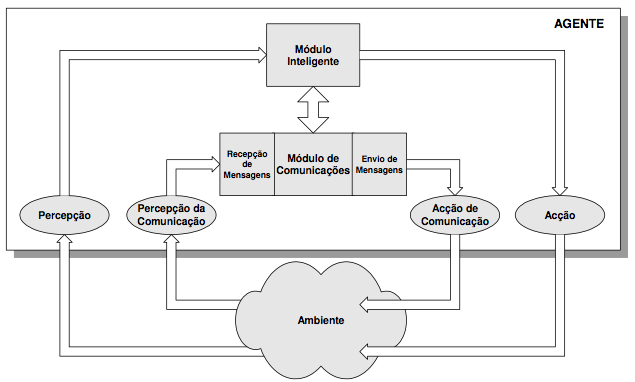
\includegraphics[scale=0.7]{figuras/arquiteturaComm.png}
\caption{Arquitetura de um agente com capacidade de comunicação.} Fonte: \cite{reisTese} \label{fig:arqComm}
\end{figure}
\FloatBarrier

\subsection{Coordenação em SMA}
\label{subsec:coosma}
O Futebol Robótico em geral e a liga de simulação em particular, constituem domínios particularmente adequados a aplicação da 
investigação realizada em metodologias de coordenação em SMA, nomeadamente no que diz respeito a coordenação
para agentes cooperativos \cite{reisTese}.

O domínio do futebol robótico é complexo, dinâmico, parcialmente cooperativo e parcialmente adverso. Existem diversos
tipos de coordenação aplicados ao domínio do futebol robótico. Neste trabalho só será descrito o tipo de coordenação que está sendo 
utilizado no desenvolvimento do modelo, porém a descrição dos diversos tipos de coordenação poderão ser encontradas 
em \citeonline{reisTese}. A coordenação pode ser:

\begin{enumerate}
\item Coordenação por Comunicação.
\item Coordenação por Percepção Inteligente,
\item Coordenação por Modelização Mútua.
\item Coordenação Estratégica.
\item Coordenação Parcialmente Hierarquica.
\end{enumerate}

O tipo de coordenação utilizada neste modelo é focada na coordenação por comunicação. A coordenação por comunicação utiliza um protocolo
que permite que os agentes possam trocar informações acerca do seu estado de mundo e outras informações úteis para a coordenação. Este 
protocolo é baseado no envio de mensagens através de um canal de comunicação entre o agente e o servidor.

A baixa largura de banda do domínio e as restrições impostas à comunicação, são fatores que tornam o futebol robótico simulado um domínio 
atraente para a aplicação de metodologias de coordenação por comunicação.

O time BahiaRT do ACSO, além de utilizar coordenação por comunicação, utiliza a coordenação estratégica. Este tipo de coordenação utiliza 
como premissa a organização dos agentes de tal forma que eles possam definir uma estratégia para um dado jogo, ou situação, composta de 
táticas e definição de papéis (tipos de jogadores) especificando o comportamento individual e coletivo dos agentes.

A construção de agentes capazes de balancear a reatividade com a capacidade de deliberação individual e social são fundamentais 
para que os agentes realizem a cooperação. O estado do mundo de um agente estratégico é definido como uma estrutura multi-nivel
contendo desde informações de baixo nível (incluindo as posições, velocidade e orientações dos objetos presentes no mundo), até 
informação de nível estratégico (incluindo informação temporal estratégica que irá permitir a seleção de táticas a serem utilizadas). 
Este estado de mundo é atualizado utilizando informação proveniente da percepção do agente, das comunicações recebidas (mensagens), da 
dinâmica do mundo e da predição dos efeitos das suas ações e das ações dos outros agentes.

\section{Futebol de Robôs}
\label{sec:futebolderobos}
A iniciativa RoboCup \cite{kitano95} \cite{Kitano97} é um projeto de investigação e educação internacional que tem como objetivo 
promover a investigação em Inteligência Artificial Distribuída (IAD) e Robótica Inteligente \cite{robocup}. O projeto tem como base a 
utilização de um problema padrão – o futebol robótico – onde o desenvolvimento de tecnologias para construir uma equipe de robôs 
reais ou virtuais seja capaz de participar de um desafio de futebol seguindo regras de jogo pré-especificadas.

Como forma de promover a investigação na área, foi lançado um objetivo de longo prazo: 

“No ano de 2050, uma equipe de robôs autônomos humanóides, ser capaz de vencer a 
equipe campeã do mundo de futebol, em uma partida disputada de acordo com as regras da 
FIFA.” \cite{Kitano97} 

Este objetivo é atualmente partilhado como um dos grandes desafios da área da IA e Robótica. 
Embora este desafio, à luz da ciência e tecnologia atuais, pareça altamente ambicioso, a colocação de objetivos científicos
bem definidos de longo prazo, tem sido, ao longo dos anos, uma forma de estimular o desenvolvimento científico \cite{robocup}. 
Além disso, os sub-objetivos que são colocados pela RoboCup através das ligas, convergem para alcançar o objetivo final.

\subsection{Ligas da RoboCup}
\label{subsec:ligasdarobocup}
O futebol robótico inclui diversas ligas que se dividem em dois tipos: ligas robóticas (utilizando robôs pequenos, médios e 
humanóides) e a liga de simulação. O objetivo é fazer com que cada liga se concentre nos desafios propostos, dando ênfase em 
determinados tópicos necessários para fazer com que equipes de robôs possam disputar uma partida de futebol. Por exemplo, 
na liga de simulação, a ênfase é colocada na coordenação em SMA, enquanto na liga de robôs pequenos, a ênfase é colocada no 
controle rápido e preciso dos robôs e na liga de robôs médios, os tópicos mais importantes incluem a visão computacional, 
projeto electromecânico e auto-localização dos robôs.

A RoboCup Rescue \cite{kitano99} e o RoboCup Júnior \cite{sklar02} são também outras iniciativas associadas ao futebol robótico. 
O {\it Rescue} divide-se em robótica física e simulada e tem como objetivo estimular a aplicação da investigação realizada no futebol 
robótico, a domínios socialmente mais úteis, no caso, missões de salvamento e resgate em grandes catástrofes \cite{rescue01}. Já 
a RoboCup Júnior surgiu como uma forma de estimular os mais jovens a participar da RoboCup. A OBR (Olimpíada Brasileira de Robótica) 
é um dos eventos que promovem a inclusão de jovens em idade escolar a construir e colocar em funcionamento os seus robôs para 
realizar diversas tarefas e atraí-los para a CBR (Campeonato Brasileiro de Robótica), que vem atraído a cada ano mais estudantes.

\subsection{Xadrez vs RoboCup}
\label{subsec:xadrezvsrobocup}
Um desafio semelhante colocado aos investigadores em IA no decurso das últimas 4 décadas, consistiu em 
construir um agente (programa) que fosse capaz de vencer o campeão mundial de Xadrez utilizando as regras oficiais da Federação
Internacional de Xadrez. Tal desafio mostrou a importância da existência de problemas padrão em que diferentes metodologias e
avanços científicos podem ser comparados. 

Diversos algoritmos de pesquisa, arquiteturas de computadores e metodologias científicas foram desenvolvidas para este domínio. 
Em Maio de 1997, o computador Deep Blue da IBM \cite{deepblue} derrotou Gary Kasparov (o campeão humano de Xadrez), figura \ref{fig:deepblue}
, utilizando as regras oficiais do Xadrez. Com esta vitória, o desafio de 40 anos da IA utilizando o Xadrez 
como domínio de aplicação ficou muito próximo de um final com sucesso. 

\begin{figure}[!htb]
\centering
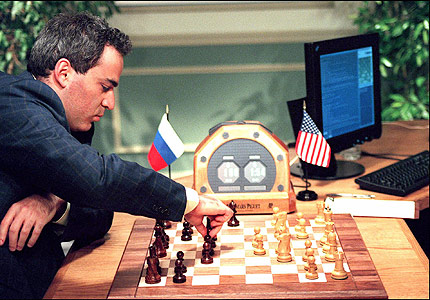
\includegraphics[scale=0.6]{figuras/deepblue.jpg}
\caption{Garry Kasparov x Deep Blue (Computador da IBM), jogando uma partida de Xadrez.} Fonte: \cite{flamencos} \label{fig:deepblue}
\end{figure}
\FloatBarrier

Uma das características que tornou o Xadrez computadorizado um problema padrão foi a facilidade que este domínio ofereceu para
a comparação de abordagens distintas, e para a avaliação do progresso científico global realizado no domínio. No entanto, com a
chegada ao final do desafio associado ao Xadrez, no mundo da IA, novos domínios e problemas padrão mais complexos e estimulantes
tornaram-se necessários. Foi neste contexto que se desenvolveu o desafio do futebol robótico como um problema padrão para a IAD 
e Robótica Inteligente.

As principais diferenças entre o domínio do Xadrez e a RoboCup podem ser visualizadas na tabela \ref{tab:xadrobocup}.

\begin{table}[!htb]

\centering

\caption{Diferenças entre as características dos domínios do RoboCup e Xadrez.} Fonte: \cite{reisTese} 

  \begin{tabular}{|c|c|c|}

    \hline
    \hline
    Caracteristicas / Domínio & Xadrez & RoboCup \\
    \hline
    Ambiente & Estático & Diamico \\
    \hline
    Mudança de Estado & Por turnos & Tempo-Real \\
    \hline
    Acessibilidade ao Estado do Mundo & Completa & Incompleta \\
    \hline
    Resultado das Ações & Determinístico & Não Determinístico \\
    \hline
    Leitura dos Sensores & Discreta (Simbólica) & Contínua (não Simbólica) \\
    \hline
    Utilização dos Atuadores & Discreta (Simbólica) & Contínua (não Simbólica) \\
    \hline
    Controle & Centralizado & Distribuído \\
    \hline
    \hline
  \end{tabular}

  \label{tab:xadrobocup}
\end{table}

A RoboCup foi desta forma projetada de forma a colocar num mundo limitado, um conjunto elevado de complexidades do mundo real, 
mantendo no entanto o custo, complexidade global e dimensão do problema, acessível aos grupos de investigação em Robótica e 
IA. Tais problemas de investigação colocados pela RoboCup de uma forma integrada, cobrem uma vasta área dos 
domínios da IA e Robótica, incluindo: coordenação, cooperação e comunicação multi-agente, arquiteturas de agentes inteligentes, 
aprendizagem, planejamento em tempo-real, decisão estratégica e tática, comportamento reativo, visão computacional, processamento
e análise de imagem, sistemas de locomoção e atuação, sistemas sensoriais, fusão sensorial em tempo-real, navegação, controle 
inteligente robótico e outros.

\subsection{Simulação 3D}
\label{subsec:simulacao3d}
A Simulação 3D de futebol de robôs da RoboCup é uma plataforma que tem como objetivo facilitar o desenvolvimento das pesquisas e 
diminuir o custo com experimentos que os robôs físicos demandam. 

A plataforma se esforça para reproduzir os desafios de 
programação de {\it Software} enfrentdos ao construir robôs físicos reais para esta finalidade. Com a utilização da simulação 3D, 
a investigação encurta o caminho para conseguir atingir a meta da Federação RoboCup de desenvolver uma equipe de robôs humanóides 
totalmente autônomos que possa vencer a equipe campeã mundial de futebol humano em 2050.

\subsection{Simspark}
\label{subsec:simspark}
SimSpark \citeonline{simspark} é um sistema de simulação multi-agente para agentes em ambiente tridimensional desenvolvido como
parte da iniciativa RoboCup. Seu objetivo é fornecer um alto grau de flexibilidade para a criação de novos tipos de simulações. 
Baseia-se em um quadro de aplicação flexível e esgota a idéia de componentes substituíveis ao longo de sua implementação. 

Em comparação com simuladores especializados, os usuários podem criar novas simulações utilizando uma linguagem de descrição de
cena. O SimSpark é uma ferramenta poderosa, pois abrange diferentes questões de investigação multi-agente, e é usado como o 
simulador oficial para a competição {\it RoboCup Simulation League}.

O {\it rcssserver3d} é o ambiente de competição oficial para o {\it Soccer Simulation League} em 3D na RoboCup. Ele implementa uma simulação
de futebol, onde duas equipes de até onze robôs humanóides podem jogar uns contra os outros. Esta configuração aparentemente 
simples, representa um desafio para os implementadores de agentes em vários níveis. 

O modelo de robô utilizado na simulação nas competições é atualmente o NAO, figura \ref{fig:naoColorido}. Contudo, a utilização de agentes
heterogeneos tem ganhado destaque na área científica, que agora querem criar modelos capazes de se adequarem a qualquer tipo de 
robô.

\begin{figure}[!htb]
\centering
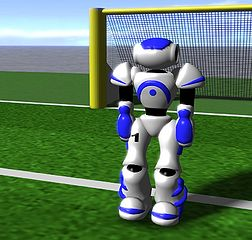
\includegraphics[scale=0.6]{figuras/naoColorido.jpg}
\caption{Simulação do Robô NAO da empresa Aldebaran Robotics feita pelo servidor oficial da liga 3D.} Fonte: \cite{SimulationLeague}. \label{fig:naoColorido}
\end{figure}
\FloatBarrier
              
\subsection{Roboviz}
\label{subsec:roboviz}
RoboViz \citeonline{roboviz} é um programa de {\it Software} projetado para avaliar e desenvolver comportamentos de agentes em sistemas 
multi-agente. RoboViz é um monitor interativo que torna o agente e informações sobre o 
estado do mundo em uma cena tridimensional. Além disso, o RoboViz fornece um design programável e funcionalidade de depuração
para os agentes que podem se comunicar através de uma rede. 

A ferramenta facilita a visualização em tempo real de agentes em execução simultânea no simulador SimSpark, fornecendo uma análise
de nível superior e visualização de comportamentos do agente, figura \ref{fig:roboviz}, que não está atualmente disponível nas 
ferramentas já existentes.

\begin{figure}[!htb]
\centering
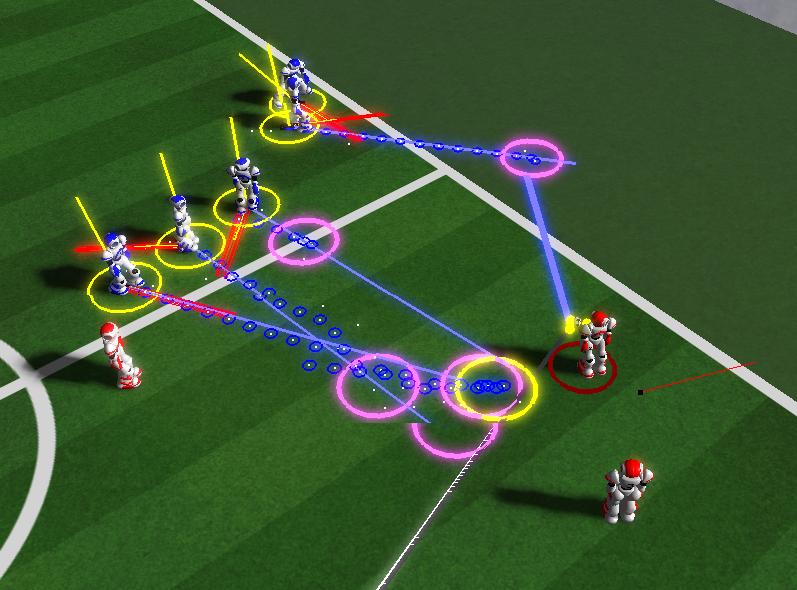
\includegraphics[scale=0.38]{figuras/roboviz.png}
\caption{Simulação em tempo real de agentes no RoboViz utilizando um plot gráfico para analise de comportamentos.} Fonte: \cite{robovizImg} \label{fig:roboviz}
\end{figure}
\FloatBarrier

\subsection{Times da Simulação 3D}
\label{subsec:times3d}
A liga de simulação 3D é composta por times que foram desenvolvidos por grupos de pesquisa de diversos países. A quantidade de
equipes que possuem times competitivos é pequena, isso se da pelo fato de que o desenvolvimento de uma equipe requer uma pesquisa
aprofundada sobre movimentação de agentes, protocolos de comunicação, planejamento e coordenação multi-agente e IAD.

Um dos fatores que facilitam grupos de pesquisa se inserirem na competição, são os códigos de times base disponibilizados por equipes para
fomentar e estimular a pesquisa no \^ambito da robótica autônoma simulada. Como por exemplo, o MagmaOffenburg \cite{magma}, um time
base cedido para a comunidade científica.

Atualmente os principais times que participam da RoboCup podem ser visualizados na tabela \ref{tab:times}.

\begin{table}[!htb]

\scalefont{0.8}
\centering
\caption{Principais times que participam da RoboCup e sua Universidade.} Fonte: \cite{SimulationLeague} 

  \begin{tabular}{|c|c|}
    \hline
    \hline
    Time & Universidade \\
    \hline
    \hline
    Apollo3D & Nanjing University of Posts and Telecommunications \\
    \hline`
    AUA3D & Anhui University of Architecture \\
    \hline
    BahiaRT & Universidade do Estado da Bahia \\
    \hline
    Bold Heart & University of Hertfordshire \\
    \hline
    cit3d & Changzhou Institute of Technology \\
    \hline
    FCPortugal & University of Aveiro/University of Minho/University of Porto \\
    \hline
    FUT-K3D & Fukui University of Technology \\
    \hline
    HfutEngine3D & HFUT \\
    \hline
    ITAndroids & Instituto Tecnologico de Aeronautica \\
    \hline
    IUIM3D & Iran University of Industries Mines (Tehran Center Branch) \\
    \hline
    KarachiKoalas & University of Technology, Sydney and Institute of Business Administration, Karachi \\
    \hline
    KylinSky3D & Hohai University Wentian College / Hohai University \\
    \hline
    L3M-SIM & Paris8 University \\
    \hline
    magmaOffenburg & Hochschule Offenburg \\
    \hline
    Miracle3D & Hefei Normal University \\
    \hline
    Mithras3D & Farzanegan Tehran \\
    \hline
    Nexus3D & Ferdowsi University of Mashhad \\
    \hline
    ODENS & Osaka Electro-Communication University \\
    \hline
    Paydar3D & Sharif University Of Technology \\
    \hline
    Rightel & University of Tehran \\
    \hline
    RoboCanes & University of Miami \\
    \hline
    Scorpius & AmirKabir University of Technology (AUT) \\
    \hline
    SEU-Jolly & Southeast University \\
    \hline
    UTAustinVilla & University of Texas at Austin \\
    \hline
    \hline
  \end{tabular}

  \label{tab:times}
\end{table}


Além dos times base, o TDP ({\it Team Description Paper}), que são descrições de cada time e artigos sobre as metodologias empregadas
em seus times, são divulgadas em simpósios e congressos, facilitando o trabalho de outras equipes e fomentando a melhoria contínua
de metodologias empregadas para resolver problemas em aberto.

Alguns dos problemas em aberto nesta liga são: como fazer com que os agentes corram, fazer 
com que agentes efetuem um passe de forma coordenada e planejada, desviar de obstáculos móveis e atuarem com sucesso em ambi\^entes dinâmicos. 
Um dos times que mais se aproxima da movimentação baseada no comportamento humano é o MagmaOffenburg \cite{dorer}, 
que por sua vez poderá ser um dos primeiros times a conseguir fazer com que o robô consiga correr.

Um outro time que ganhou destaque nas últimas competições foi o UTAustinVilla \cite{MacAlpine2}. Desenvolvido por um grupo de 
estudantes da Universidade de Austin, Estados Unidos, coordenado por Peter Stone, pesquisador renomado na área de robótica. 
Uma das principais características que determinaram o seu sucesso foi a sua movimentação omnidirecional com capacidade de 
se manter estável mesmo colidindo com outros agentes.

O time FCPortugal \citeonline{fcportugal} desenvolvido pelo grupo de pesquisa da Universidade do Porto, Portugal, terceiro lugar na simulação 3D da 
RoboCup 2013, teve como diferencial o seu super chute, capaz de alcançar até 20 metros, mais da metade do campo utilizado pelo servidor 
Simspark. Apesar de ser um chute estático, o seu alcance é fruto da otimização do {\it script} utilizado na perna que realiza o chute.

Na RoboCup de 2013, o time vencedor da simulação 3D foi o Apollo3D \cite{apollo3d}. Uma das principais contribuições que o 
grupo de pesquisa que desenvolveu o Apollo3D vem dispondo a comunidade científica é o seu código fonte.

A maioria dos times hoje utilizam uma movimentação omnidirecional e dinâmica, onde suas poses são calculadas e alcançadas através de 
modelos matemáticos utilizando cinemática inversa. Tais modelos substituiram a movimentação estática, que dificultava a realização de 
jogadas e comportamentos devido o fato de que o ambiente é dinâmico e contínuo. 


\section{Planejamento de trajet\'oria}
\label{sec:planejamentodetrajetorias}
O objetivo principal do planejamento de trajetória é a construção de algoritmos para automatizar o movimento de robôs, 
peças e outros ambientes que utilizam objetos geométricos arbitrários. Uma tarefa básica é mover um robô em seu ambiente de trabalho 
a partir de uma posição e orientação para outra posição e orientação desejada, sem o robô bater em obstáculos. O planejamento de trajetória
tem aplicações tanto dentro, como fora da área de robótica.

O problema de navegação mais básico é mover um robô modelado como um ponto no espaço através de um ambiente bidimensional com vários
itens proibidos (ou obstáculo). O obstáculo é considerado uma região em que o robô não pode entrar. O modelo é cinemático, o que significa
que a única limitação é que o robô tem de se mover ao longo de uma trajetória contínua.

O robô é modelado como um ponto no espaço de configuração, em vez de espaço de trabalho. Uma configuração é uma especificação
do local (localização e orientação) do robô em relação ao meio ambiente e o espaço de configuração é o conjunto de todas as configurações
possíveis \cite{achoset}.

Realizar o planejamento apresenta um maior nível de complexidade quando o robô tem muitos graus de liberdade e orientação. Um robô 
guia pode passar por um espaço com uma certa posição e orientação, e atinge um obstáculo se fosse em uma orientação diferente. Isso 
aumenta a complexidade dos algoritmos para planejamento de trajetória. Além disso, podem existir obstáculos móveis no ambiente, 
aumentando ainda mais a complexidade da busca de uma trajetória eficiênte, sem que haja colisão.

O exemplo clássico de planejamento de trajetória é o problema do mecanismo de enfileiramento \cite{bsharir}: 
mover um piano através de uma casa sem colidir com outros objetos na casa (ou a própria casa). Considerando somente a 
geometria dos objetos e não as forças que atuam sobre o piano, como a gravidade .

Estendendo a analogia, o piano é suposto ter motores infinitamente fortes e infinitamente pequenos. Portanto, o problema do motor 
de piano só lida a circulação de uma forma geométrica ao longo de um caminho que é contínuo no espaço através de uma atmosfera.

Existem diversos algoritmos que tratam da navegação de agentes autônomos, sendo que um dos primeiros é descrito no livro de
Inteligência Artificial de Russell e Norvig, o algorítmo A* \cite{brussel}. Ele busca o caminho em um grafo de
um vértice inicial até um vértice final, é a combinação de aproximações heurísticas como do algoritmo {\it Best-first Search} e da
formalidade do Algoritmo de Dijkstra (DIJKSTRA, 1959). 

A partir do algoritmo A*, surgiram derivações como o R* \cite{plikhachev}, que depende muito menos da qualidade da função heurística, 
evitando mínimos locais e resolvendo o problema de planejamento de toda uma série de pesquisas de curto alcance.
    %---------- Segundo Capitulo ----------
\chapter{Modelo de mapeamento e planejamento de trajetória}
\label{chap:desenv}
O objetivo deste capítulo é descrever o modelo desenvolvido, apresentando uma descrição de todo o processo envolvido no 
desenvolvimento, especificando a arquitetura do modelo, a metodologia utilizada para desenvolver o projeto e os trabalhos 
correlatos.

\section{Trabalhos relacionados}
\label{sec:trabalhosrelacionados}
Visando identificar os principais trabalhos desenvolvidos para planejar trajetória, foram realizados alguns estudos no âmbito 
do planejamento de trajetória e predição de colisão para especificar melhor o domínio no qual o trabalho foi desenvolvido e 
realizar um estudo comparativo das diferenças do modelo proposto e os pesquisados. A pesquisa não se limitou ao domínio do futebol 
de robôs e \`a simulação.

Existem muitas abordagens e modelos para planejamento de trajetória, porém a maioria dos modelos foram desenvolvidos para serem 
utilizados em ambientes estáticos, e este modelo foi desenvolvido para ser utilizado em ambiente contínuo e não determinístico. 
Alguns modelos utilizam uma abordagem em cluster, onde utilizam um banco de dados para treinamento e aprendizagem com o objetivo 
de encontrar trajetórias \cite{Jetchev}, ou para realizar agrupamentos de trajetórias para identificação de padrões de movimento 
\cite{sungFeldman}. Na simulação 3D não é viável e eficiênte utilizar grandes quantidades de dados e ter tempos de processamento 
acima de $0.02$ segundos, tempo máximo para o agente tomar uma decisão.

\citeonline{guo2009combination} desenvolveu um modelo que capta as imagens e realiza um treinamento para busca do melhor caminho filtrando o erro entre a 
predição e o ambiente real. O mapeamento do modelo é realizado supondo áreas definidas como quadrados, onde o agente se movimenta de 
um por um, com o objetivo de evitar colisões.

Algumas abordagens híbridas para planejamento de trajeória utilizam uma combinação de planejamento de passo, algoritmo de busca e 
checagem de colisão \cite{hamasaki}\cite{phornungfootstep}. Estes modelos utilizam um mapa 2D composto por células de tamanho igual que são 
marcadas como livres ou ocupadas. Basicamente o modelo primeiro realiza um método recursivo de avaliação de colisão e depois utilizam o 
algoritmo de busca para encontrar o melhor caminho sem possibilidade de colisão.

O modelo proposto neste trabalho tem como base a busca de uma trajetória livre de colisão, realizando o mapeamento de possíveis trajetórias e verificando 
possíveis colisões a partir da predição da trajetória dos obstáculos móveis. Além de encontrar a melhor trajetória, foi utilizado uma 
combinação de um modelo de movimentação omnidirecional do BahiaRT, que já estava implementado, aumentando ainda mais a eficácia da navegação 
do agente no ambiente.
 
Por fim, o desenvolvimento e pesquisa de abordagens para ambiêntes dinâmicos ainda é considerado um grande desafio, pois requer modelos 
em tempo real, preditivos, com processamento de imagens e de padrões de comportamento eficiêntes e ao mesmo tempo que garantam a segurança 
dos envolvidos no ambiente. Por este motivo, o trabalho está sendo desenvolvido utilizando como domínio o futebol de robôs.

\section{Proposta Metodológica}
\label{sec:proposta}
O desenvolvimento deste projeto foi dividio em 5 etapas apresentadas na figura \ref{fig:metodologia}.

\begin{figure}[H]
\centering
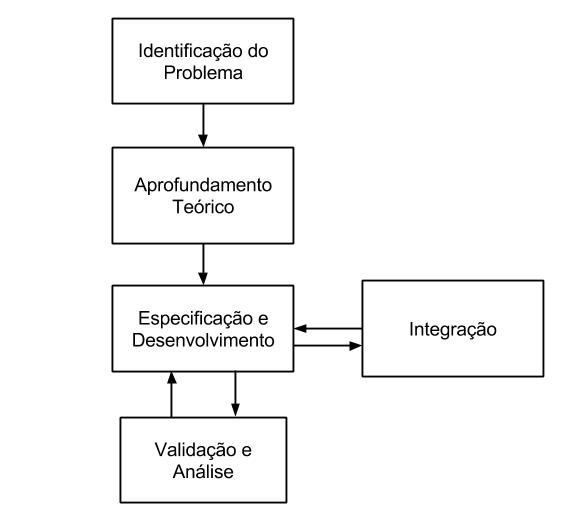
\includegraphics[scale=0.4]{figuras/metodologia.jpg}
\caption{Etapas da metodologia do projeto.} 
\label{fig:metodologia}
\end{figure}
\FloatBarrier

Na etapa inicial, definida como "Identificação do Problema", foi realizado um estudo do ambiente simulado 3D, através da 
especificação PEAS\cite{brussel} no domínio de futebol de robôs para identificar quais fatores influenciam na 
tomada de decisão do agente na identificação da melhor trajetória a ser seguida até o objetivo sem que haja colisão.

Na etapa seguinte, "Aprofundamento Teórico", foi realizado um estudo sobre planejamento de trajetória, planejamento multi-agente, 
coordenação multi-agente, predição de colisão e mapeamento de ambientes dinâmicos. Esta etapa teve como objetivo identificar 
trabalhos relacionados ao problema identificado na etapa anterior. O resultado do estudo foi descrito na Seção \ref{sec:trabalhosrelacionados}.

A etapa de "Especificação e Desenvolvimento" teve como base o desenvolvimento do modelo a partir da especificação dos requisitos e da 
modelagem da solução utilizando o time BahiaRT. Em conjunto com essa etapa, foi realizada a etapa de "Integração", fazendo as modificações 
necessárias no código do time BahiaRT e integrando o modelo desenvolvido.

Finalmente, na etapa "Validação e Análise", foi realizada uma especificação da metodologia de teste, da instalação do ambiente de teste e 
executados os testes para validar o modelo desenvolvido. Onde a validação foi realizada utilizando uma aplicação de passe 
desenvolvido para avaliar a eficácia das trajetórias encontradas, rodando o time com os melhores times da liga de simulação 3D dos últimos anos. E 
nesta mesma etapa, foram coletados os resultados obtidos, retornando a etapa anterior para corrigir falhas de desenvolvimento.

\section{Arquitetura do modelo}
\label{sec:arquitetura}
A arquitetura da aplicação de passe desenvolvida para validar o modelo proposto pode ser vista na figura \ref{fig:arquitetura}.

\begin{figure}[H]
\centering
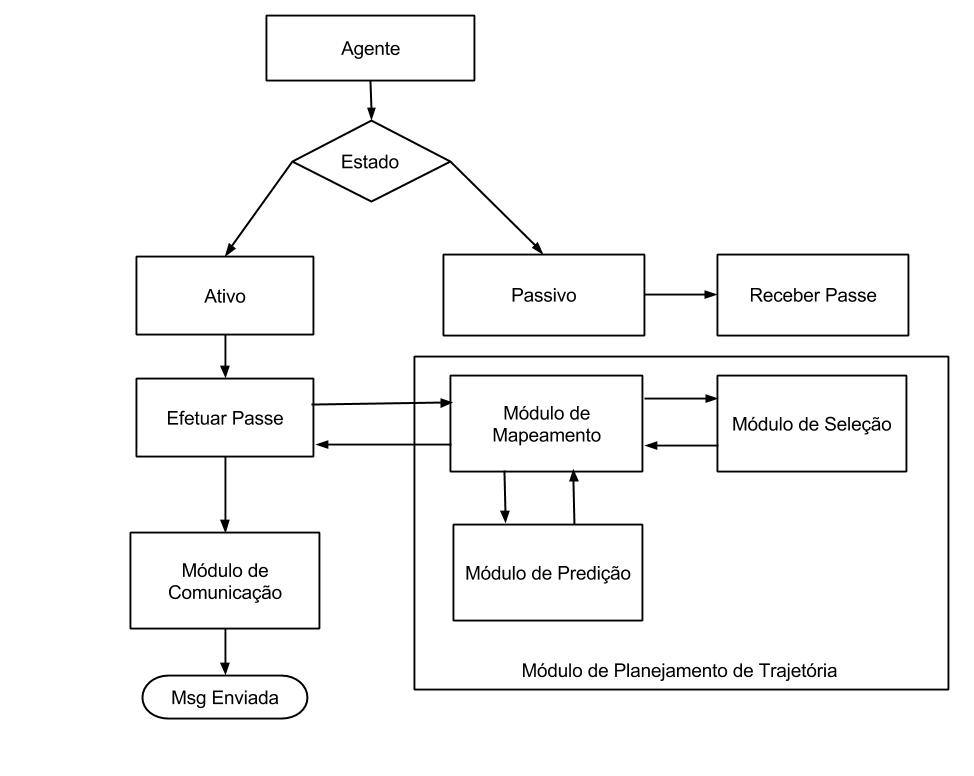
\includegraphics[scale=0.45]{figuras/ArquiteturaModelo.jpg}
\caption{Arquitetura do projeto desenvolvido integrado a um modelo de passe desenvolvido para validação.} 
\label{fig:arquitetura}
\end{figure}
\FloatBarrier

Nesta arquitetura, um agente pode estar em estavo ativo, ou passivo. Um agente em estado ativo, é designado como um agente que está com 
pose de bola, ou lutando pela pose de bola. Já os agentes passivos são considerados agentes de suporte, que ficam em posições estratégicas. No 
momento em que um agente está em estado ativo e com pose de bola, ele verifica a possibilidade de efetuar um passe.

O passe só é realizado se obedecer as seguintes regras:

\begin{enumerate}
 \item O oponente mais próximo deve estar a $4$ metros de distância.
 \item Deve existir pelo menos $1$ agente aliado em uma posição estratégica.
 \item O agente aliado que vai receber um passe não deve estar caído.
 \item O agente aliado que vai receber um passe não deve estar marcado por agentes oponentes.
 \item O agente que vai efetuar o passe deve estar em estado ativo e com a pose da bola.
 \item Deve existir uma trajetória confiável para onde o agente vai chutar a bola.
\end{enumerate}

Inicialmente é realizado o mapeamento e a busca das melhores trajetórias para lançar a bola. Depois é realizada uma busca dos melhores 
jogadores para receber o passe com base nas trajetórias. Em seguida o módulo de passe verifica dentre as trajetóris mapeadas e o 
posicionamento dos agentes aliados qual é a melhor trajetória para se obter sucesso no passe da bola. 

Quando a trajetória é escolhida, o agente envia uma mensagem {\it broadcast} avisando a posição em que a bola vai ser lançada e quem é o agente aliado que deve se deslocar para receber o passe. Quando os agentes recebem a mensagem, eles verificam se um passe está sendo realizado e quem é o agente escolhido 
para receber a bola. Por fim, o escolhido se deslocará para a posição estratégica que lhe foi comunicada.

O sucesso do passe depende não somente da aplicação desenvolvida, mas também do chute que vai ser realizado, levando em consideração os 
fatores tempo (tempo que o agente leva para chutar) e força (força aplicada pelo chute sobre a bola).

\section{Mapeamento das trajetórias}
\label{sec:map}
O mapeamento das trajetórias é realizado a partir da construção de um mapa de grade 2D, composto por células de tamanho igual 
que é projetado em segmentos em linhas $k$ do centro da trajetória. A construção do mapa leva em consideração as limitações do 
campo e o posicionamento do agente que vai calcular a melhor trajetória para alcançar o seu objetivo.

\begin{figure}[H]
\centering
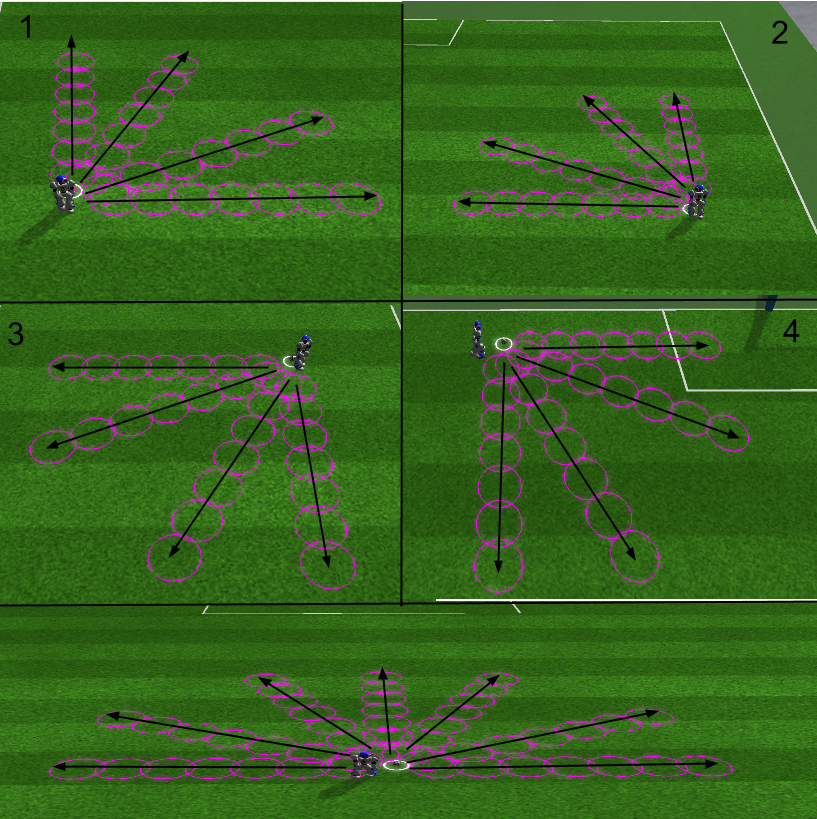
\includegraphics[scale=0.4]{figuras/Mapeamento.png}
\caption{Imagem do plot realizado pelo Roboviz representando os 5 tipos de mapeamento que é realizado pelo modelo desenvolvido.} 
\label{fig:mapeamento}
\end{figure}
\FloatBarrier

Para cada região do campo, foi definido um tipo de mapeamento, totalizando 5 tipos de mapeamento que são ilutrados na 
figura \ref{fig:mapeamento}. O objetivo foi evitar que regiões que não estavam dentro do campo fossem mapeadas e a quantidade
de células a serem verificadas fosse a menor possível, já que todo o processo de mapeamento e predição de trajetória deve ser 
feito em menos de $0.02$ segundos, que é o tempo de processamento mínimo do agente simulado 3D utilizado para desenvolvimento 
do modelo. 

Cada célula possui um conjunto de informações que são utilizadas no processo de predição da trajetória. No mapeamento de uma 
célula, apenas a posição e o número da célula são armazenados, sendo que o número representa a trajetória. As outras informações
da célula são incluídas no processo de verificação da presença de obstáculos que será descrito na próxima seção.

O diagrama de classe da célula pode ser visto na figura \ref{fig:celula}.

\begin{figure}[!htb]
\centering
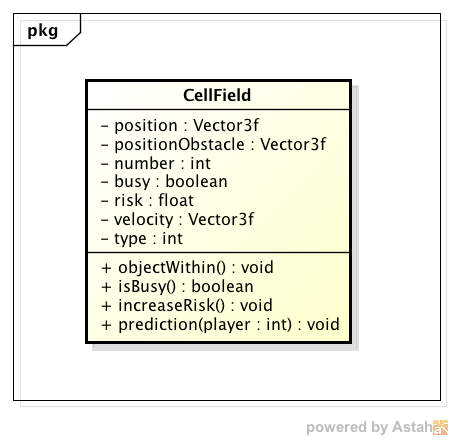
\includegraphics[scale=0.8]{figuras/celula.png}
\caption{Diagrama da classe CellFied utilizado no modelo para representar uma únidade do mapeamento.}
\label{fig:celula}
\end{figure}
\FloatBarrier

\section{Verificação da presença de obstáculos}
\label{sec:verifobstaculos}
A verificação da presença de obstáculos é feita logo após o processo de mapeamento das trajetórias. O modelo levou em consideração 
que os agentes aliados não são considerados obstáculos por conta do processo de coordenação e planejamento multi-agente que é 
realizado através do protocolo de comunicação utilizado pelo BahiaRT. Neste processo de coordenação, quando o agente encontrar a 
melhor trajetória, ele enviará uma mensagem através do canal de comunicação para todos os agentes aliados, informando a trajetória e 
outras informações que fazem parte do seu estado de mundo. O objetivo é atualizar todos os agentes sobre o estado atual do 
agente ativo.

\begin{algorithm}[!htb]
\caption{Algoritmo para verificação da presença de obstáculos}

\begin{algorithmic}[3.1]
\For{k}{1}{n}
  \For{i}{2}{11}
  
  \State $map[k].prediction(agent[i])$ \Comment{Realiza a predição de colisão}
  
  \If {$!map[k].isBusy()$}
    
    \If {$map[k].objectWithin(agent[i].position)$}
     \If {$agente[i].conf > minReliability $}
     
     \State {$map[k].velocity \gets  agent[i].velocity$} \Comment{Armazena a velocidade}
     \State {$map[k].positionOB \gets  agent[i].position$} \Comment{Armazena a posição}
     \State {$map[k].type \gets  OPPONENT$} \Comment{Armazena o tipo de obstáculo}
     \State {$map[k].busy \gets  true$} \Comment{Define a célula como ocupada}
     \State {$map[k].IncreaseRisk()$} \Comment{Incrementa o risco}
     
     \EndIf
    \EndIf
  \EndIf
  \EndFor
\EndFor
\end{algorithmic}
\end{algorithm}

No processo de verificação da presença de obstáculos, algoritmo 1, se uma célula estiver ocupada por um 
obstáculo, as informações desse obstáculo serão armazenadas. Neste processo, a posição do obstáculo, a velocidade e o tipo 
de obstáculo são armazenados na célula. Como neste domínio, apenas os agentes oponentes são considerados obstáculos, só 
existirão obstáculos de um tipo, que são os oponentes. Além dessas informações, uma taxa que indica o risco da célula é 
incrementada para indicar posteriormente se a trajetória é viável.

Cada agente possui informações dos oponentes que são utilizadas para verificar a presença dos obstáculos. Estas informações 
possuem uma taxa de confiabilidade que representa o quanto essas informações estão atualizadas. Neste processo de verificação, 
apenas os agentes oponentes que possuem no mínimo $80\%$ de confiabilidade são levados em consideração.

%\section{Calculo da velocidade dos obstáculos}
\section{Determinação da trajetória de objetos dinâmicos em ambientes ruidosos}
\label{sec:calcvel}

Para calcular a velocidade e direção dos obstáculos foi desenvolvido um modelo que filtra o ruído posicional (oscilações fortes da posição 
do objeto visto em torno da sua trajetória real) e calcula a velocidade vetorial e a escalar do objeto com poucas oscilações.

Para isso, um vetor é estendido desde a posição filtrada em cada ciclo, para o futuro, para predizer a posição futura do objeto.
Ao invés de calcular a média das velocidades, foi utilizado uma função que utiliza mínimos quadrados \cite{minQuad} 
para encontrar um valor coerente com o movimento do objeto.

Seja $n$ uma sequencia ordenada de $N$ valores numericos $n_{i},\: i=1,2,\ldots,N$.
Denotodo por $S_{a,b}(n)$ o operador que extrai uma subsequência $s=\{n_{a},n_{a+1},\ldots,n_{b-1},n_{b}\}$
da sequência $n$, sempre que $a\leq b$. Sejam $x_{i}$ e $y_{i}$
as coordenadas medidas de um objeto rastreado num plano no instante
$t_{i},\: i\geq0$. A figura \ref{fig:Sequ=0000EAncia-de-pontos-medidos}
demonstra uma sequência de pontos medidos de um objeto monitorado
pelo agente no campo de futebol, que foi localizado quando estava
parado na esquerda do gráfico e começou a se movimetar para a direita
fazendo uma trajetória complexa, que inclui um giro de $360$ graus.

\begin{figure}[!htb]
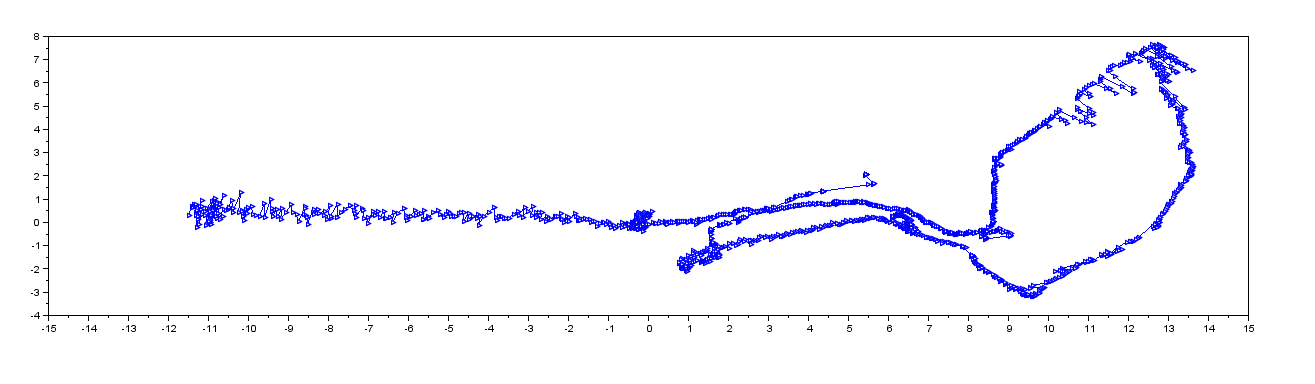
\includegraphics[scale=0.45]{figuras/fig_pontos_medidos}
\caption{\label{fig:Sequ=0000EAncia-de-pontos-medidos}Sequência de pontos
medidos de um objeto monitorado pelo agente no campo de futebol }
\end{figure}

Vale notar que independentemente do sistema sensorial utilizado, existirá
uma diferença entre o ponto medido $p_{i}=(x_{i},y_{i})$ e o ponto
onde realmente se encontra o objeto rastreado nesse instante $P_{i}=(X_{i},Y_{i})$.
Em ambientes simulados é possível realizar experimentos e registrar as
posições reais do alvo em intervalos de tempo discretos $t_{k}$ para
$k=1,2,\ldots,i$, isto é, coletando a trajetória real e medida
através de séries temporais $P=\left\{ P_{1},P_{2},\ldots,P_{i}\right\} $
e $p=\left\{ p_{1},p{}_{2},\ldots,p_{i}\right\} $. A figura \ref{fig:pontossemfiltro}
demonstra o resultado obtido em um dos experimentos, onde o objeto
foi localizado na esquerda do gráfico e começou a se movimentar para
a direita. A cor vermelha representa os pontos reais e a cor
azul os ponto medidos. 

\begin{figure}[!htb]
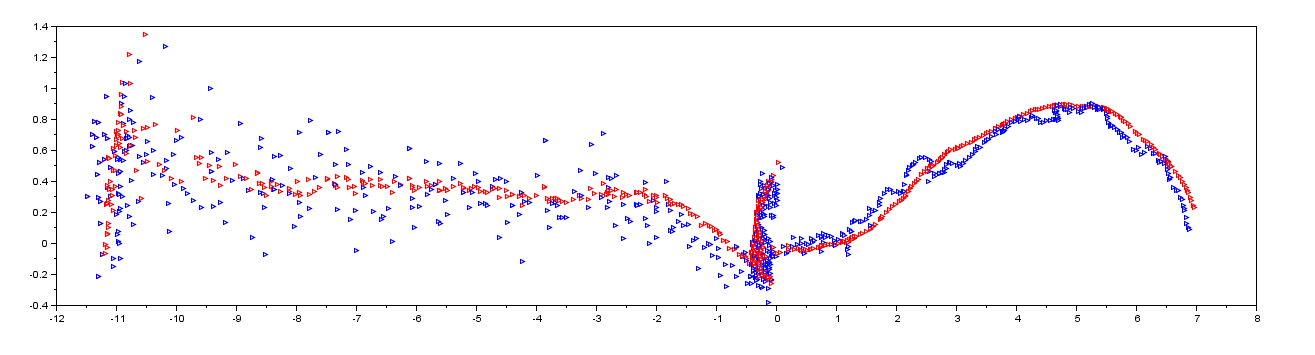
\includegraphics[scale=0.45]{figuras/fig_pontos_medidos_e_reais}
\caption{Sequência de pontos medidos e estimados de um objeto monitorado pelo agente
no campo de futebol }
\label{fig:pontossemfiltro}
\end{figure}


Note que a distância entre a posição medida $p_{i}$ e a posição real
$P_{i}$ do objeto, resultado do ruído inerente do sistema de medição,
varia com o tempo o que indica que o sistema sensorial em teste é
autoajustado, mas que mesmo assim nunca desaparece. A intensidade
do ruído posicional instantâneo vem dada por $r_{i}=\left\Vert p_{i}-P_{i}\right\Vert $
onde o operador $\left\Vert \cdot\right\Vert $ representa a norma
euclideana do vetor argumento.

Desde o ponto de vista de filtragem de ruído, o resultado relevante
são os últimos $u$ instantes da trajetória, designados como trajetórias
recentes no instante $i$, e denotados por $\Pi_{i}=S_{i-u,i}(P)=\left\{ P_{i-u},P_{i-u+1},\ldots,P_{i-1},P_{i}\right\} $
e $\pi_{i}=S_{i-u,i}(p)=\left\{ p_{i-u},p_{i-u+1},\ldots,p_{i-1},p_{i}\right\} $. 

Considerando que qualquer trajetória pode ser aproximada por uma sucessão
de segmentos de trajetórias lineares, foi utilizado o método dos
mínimos quadrados para estimar uma aproximaçao mais confiável $\tilde{P}_{i}$
da posição real do alvo no instante $i$, e com isto poder estimar
sua direção e velocidade absoluta utilizando um ponto estimado no
passado $\tilde{P}_{i-lag}$, com $lag\geq1$. A hipótese principal
do estudo é a base provada do método dos mínimos quadrados segundo
o qual $\left\Vert p_{i}-P_{i}\right\Vert \geq\left\Vert \tilde{P}_{i}-P_{i}\right\Vert $,
em média \cite{minQuad}. 

O procedimento utilizado foi o seguinte:
\begin{enumerate}
\item Obter a posição filtrada $\tilde{P}_{i}$ através de duplo ajuste
com mínimos quadrados supondo os resultados com as primeiras derivadas
das funções obtidas em cada ajuste, isto é

\begin{enumerate}
\item Cálculo dos coeficientes $a_{xy},b_{xy}$ da reta $y=a_{xy}+b_{xy}x$,
utilizando mínimos quadrados com os últimos $u-1$ pontos filtrados
$\left(\tilde{x}_{j},\tilde{y}_{j}\right),\: j=i-u,\ldots i-1$ e
o ponto medido$\left(x_{i},y_{i}\right)$. 
\item Cálculo dos coeficientes $a_{yx},b_{yx}$ da reta $x=a_{yx}+b_{yx}y$,
utilizando mínimos quadrados com os últimos $u-1$ pontos filtrados
$\left(\tilde{y}_{j},\tilde{x}_{j}\right),\: j=i-u,\ldots i-1$ e
o ponto medido $\left(y_{i},x_{i}\right)$.
\item Cálculo de dois pontos no presente (instante $i$) , $p_{1,i}=\left(x_{1,i},y_{1,i}\right)$
e $p_{2,i}=\left(x_{2,i},y_{2,i}\right)$, da forma
\[
x_{1,i}=x_{i}
\]
\[
y_{1,i}=a_{yx}+b_{yx}x_{i}
\]
\[
x_{2,i}=a_{xy}+b_{xy}y_{i}
\]
\[
y_{2,i}=y_{i}
\]

\item Cálculo do ponto mais provável no presente (instante $i$) $\tilde{P}_{i}=\left(\tilde{x}_{i},\tilde{y}_{i}\right)$
a partir dos 2 pontos acima, utilizando como peso a primeira derivada,
da forma
\[
\tilde{P}_{i}=\left(\frac{1}{b_{xy}+b_{yx}}\right)\left(b_{yx}p_{1,i}+b_{xy}p_{2,i}\right)
\]

\end{enumerate}
\item Obter a direção de movimento mais provável e a velocidade absoluta
do objeto utilizando novamente mínimos quadrados e diferenças finitas,
isto é

\begin{enumerate}
\item Cálculo dos coeficientes $a_{xy},b_{xy}$ da reta $y=a_{xy}+b_{xy}x$,
utilizando mínimos quadrados com os últimos $u$ pontos filtrados
$\left(\tilde{x}_{j},\tilde{y}_{j}\right),\: j=i-lag,\ldots i$. 
\item Cálculo dos coeficientes $a_{yx},b_{yx}$ da reta $x=a_{yx}+b_{yx}y$,
utilizando mínimos quadrados com os últimos $u$ pontos filtrados
$\left(\tilde{y}_{j},\tilde{x}_{j}\right),\: j=i-lag,\ldots i$.
\item Cálculo de dois pontos no passado (instante $i-lag+1$) , $p_{1,i-lag+1}=\left(x_{1,i-lag+1},y_{1,i-lag+1}\right)$
e $p_{2,i-lag+1}=\left(x_{2,i-lag+1},y_{2,i-lag+1}\right)$, da forma
\[
x_{1,i-lag+1}=\tilde{x}_{i-lag+1}
\]
\[
y{}_{1,i-lag+1}=a_{yx}+b_{yx}x_{1,i-lag+1}
\]
\[
y_{2,i-lag+1}=\tilde{y}_{i-lag+1}
\]
\[
x_{2,i-lag+1}=a_{xy}+b_{xy}y_{2,i-lag+1}
\]

\item Cálculo do ponto médio no passado (instante $i-lag+1$) $\hat{P}_{i-lag+1}$
a partir dos 2 pontos no passado calculados acima, isto é,
\[
\hat{P}_{i-lag+1}=0.5\left(p_{1,i-lag+1}+p_{2,i-lag+1}\right)
\]

\item Cálculo de dois pontos no presente (instante $i$) , $p_{1,i}=\left(x_{1,i},y_{1,i}\right)$
e $p_{2,i}=\left(x_{2,i},y_{2,i}\right)$, da forma
\[
x_{1,i}=\tilde{x}_{i}
\]
\[
y{}_{1,i}=a_{yx}+b_{yx}x_{1,i}
\]
\[
y_{2,i}=\tilde{y}_{i}
\]
\[
x_{2,i}=a_{xy}+b_{xy}y_{2,i}
\]

\item Cálculo do ponto médio no presente (instante $i$) $\hat{P}_{i}$
a partir dos 2 pontos no presente calculados acima, isto é,
\[
\hat{P}_{i}=0.5\left(p_{1,i}+p_{2,i}\right)
\]

\item Cálculo do vetor velocidade no presente (instante $i$), $v_{i}=\left(v_{x,i},v_{y,i}\right)$,
tal 
\[
v_{i}=\frac{\hat{P}_{i}-\hat{P}_{i-lag+1}}{t_{i}-t_{i-lag+1}}
\]

\item Cálculo da velocidade escalar no presente (instante $i$), $V_{i}=\left\Vert v_{i}\right\Vert $.
\item Cálculo do vetor de direçao no presente (instante $i$), $d_{i}={\displaystyle \frac{1}{\left\Vert v_{i}\right\Vert }}v_{i}$.\end{enumerate}
\end{enumerate}


Com o algoritmo para filtrar o ruído posicional e calcular a velocidade vetorial e escalar do agente, foi possível estimar os 
pontos de colisão com maior precisão, auxiliando na escolha da melhor trajetória.

\section{Predição de colisão dos obstáculos}
\label{sec:calctrajetoria}
Neste modelo, além de levar em consideração a presença de obstáculos nas trajetórias, é realizado um processo de predição de 
deslocamento dos obstáculos que estão em regiões próximas com o objetivo de predizer se o obstáculo irá estar na trajetória 
no mesmo instante em que o agente estiver se deslocando para o ponto objetivo, ou se tiver chutado a bola na trajetória escolhida 
e ela estiver se deslocando até o ponto objetivo.

O principal objetivo da predição é evitar que o agente ou a bola colida com o obstáculo no momento em que estiver se deslocando 
em direção ao objetivo. A partir desta análise, se um agente oponente levar um tempo menor para chegar ao ponto $P$ da trajetória, 
que o agente aliado, ou a bola, então o risco deste ponto aumenta, sendo que cada ponto é considerado como a célula da trajetória, 
e que para cada célula, são verificados os agentes oponentes próximos desta trajetória que foi mapeada.

O calculo da predição do deslocamento do agente oponente é realizado com a velocidade do agente calculada e a distância entre o 
oponente e a trajetória:

\begin{equation}
D = A - B 
\end{equation}
\begin{equation}
T = \frac {D} {V}
\end{equation}

onde $D$ é a distância do ponto $A$ ao ponto $B$, $V$ é a velocidade do oponente e $T$ é o tempo que o agente
levaria até chegar ao ponto $B$, levando em consideração que a velocidade é constante.

O cálculo do ponto previsto é descrito como:

\begin{equation}
  P = Po + V * T 
\end{equation}

onde $P$ é o ponto previsto, $Po$ é a posição atual, $V$ é a velocidade e $T$ é o tempo em que estou estimando a posição. O 
algoritmo resumido pode ser visto abaixo no algoritmo 2.

\begin{algorithm}[!htb]
\label{alg:prediction}
\caption{Algoritmo para predição de colisão}
\begin{algorithmic}[3.2]
\Function{Prediction}{agent}
  \If {$agent.conf < minReliability$}
    \State \Return
  \EndIf
  
  \State {$ballTime \gets distanceBallToCellField / velBall$}
  \State {$meTime \gets distanceMeToCellField / velMe$}
  \State {$deltaS \gets agent.distanceToCellField$}
  \State {$agentSpeed \gets agent.velocity$}
  
  \If {$agentSpeed <= 0 $}
    \State $agentSpeed \gets 0.1$
  \EndIf
  
  \State {$deltaT \gets deltaS / agentSpeed$}
  \State {$estimedPostition \gets agent.position + agent.velocity * deltaT$}
  
  \If{$objectWithin(estimedPostition)$}
  
    \If{$((deltaT+TIME_PERCEPTION) < ballTime) || (deltaT+TIME_PERCEPTION < meTime)$}
      \State $increaseRisk()$
    \EndIf
    
    
    \If {$(maxVelocityAgent - agentSpeed) < minVel$}
      \State $increaseRisk()$
      \State $increaseRisk()$
    \Else
      \State $increaseRisk()$
    \EndIf
    
  \EndIf
\EndFunction
\end{algorithmic}
\end{algorithm}

\section{Critério do descarte de obstáculos}
\label{sec:descarte}
O modelo levou em consideração apenas os obstáculos que possuíam informações atualizadas e que estavam próximos da trajetória. O 
objetivo foi evitar utilizar obstáculos que não possuem nenhum risco para a predição da trajetória.

    

    \chapter{Validação e Resultados Obtidos}
\label{chap:resultados}
O objetivo deste Capítulo é descrever todo o processo de coleta de indicadores e validação do modelo desenvolvido. Este 
Capítulo está dividido em 4 Seções.

A Seção \ref{sec:metodologia} descreve a metodologia de teste utilizada, os componentes utilizados no 
ambiente de teste e os {\it frameworks} utilizados para realizar os testes do modelo.

Na Seção \ref{sec:cenarios} são descritos os cenários definidos como casos de teste para realizar a validação do modelo.

A Seção \ref{sec:metricas} descreve quais foram as métricas utilizadas para validar o modelo.

Por fim, a Seção \ref{sec:resultados} descreve os resultados obtidos no processo de validação do modelo, as considerações e 
a importância dos resultados obtidos com o desenvolvimento do modelo.

\section{Metodologia de Teste}
\label{sec:metodologia}
A realização dos testes se deu através de um ambiente real de competição. O ambiente foi montado utilizando 4 computadores
conectadas através de um {\it switch}. As configurações dos componentes utilizados pode ser vista na tabela \ref{tab:configambiente}.

\begin{table}[!htb]

\scalefont{0.8}

\centering

\caption{Configuração dos computadores utilizados no ambiente de teste para coleta dos resultados.}.

  \begin{tabular}{|c|c|}

    \hline
    \hline
    Programa utilizado & Configuração do componente \\
    \hline
    \hline
    Time BahiaRT  & Notebook DELL Core i7, RAM-8GB, HD-1TB , Placa de vídeo - 2GB  \\
    \hline
    Time Oponente  & Notebook DELL Core i7, RAM-8GB, HD-1TB , Placa de vídeo - 2GB \\
    \hline
    Simspark  & Notebook DELL Core i7, RAM-8GB, HD-1TB , Placa de vídeo - 2GB \\
    \hline
    Roboviz & Notebook DELL Core i7, RAM-8GB, HD-1TB , Placa de vídeo - 2GB \\
    \hline
    \hline
  \end{tabular}

  \label{tab:configambiente}
\end{table}

Para realizar a validação do modelo, foi necessário instalar e configurar o Simspark e o RoboViz, que são plataformas padrões
para a simulação 3D do futebol de robôs. O servidor Simspark foi instalado em um computador e o RoboViz que é onde a simulação
do ambiente é renderizada, foi instalada em outro computador. Os outros 2 computadores, que são as máquinas clientes onde os 
binários dos times foram executados, são máquinas que possuiam apenas o sistema operacional instalado, que neste caso foi utilizado 
o {\it Ubuntu 12.04 LTS}. A arquitetura do ambiente pode ser vista através da figura \ref{fig:arquiteturaAmbiente}.

\begin{figure}[!htb]
\centering
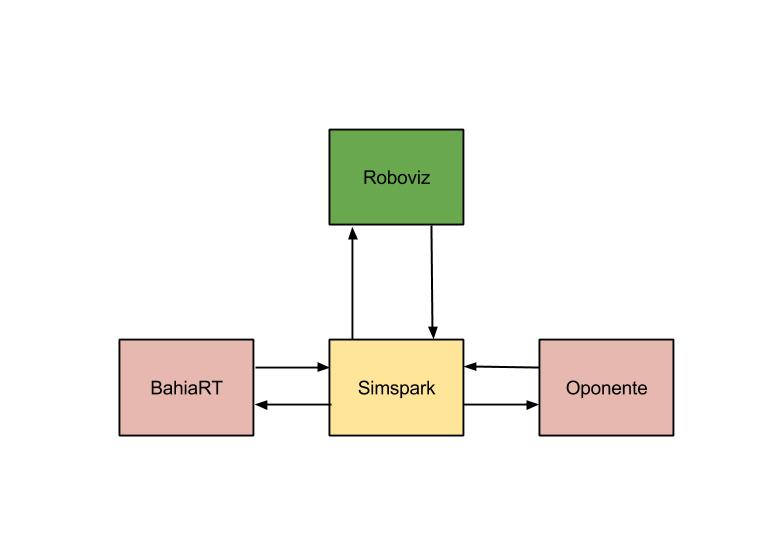
\includegraphics[scale=0.50]{figuras/ambienteTeste.jpg}
\caption{Arquitetura do ambiente de teste utilizado para coletar os resultados.} 
\label{fig:arquiteturaAmbiente}
\end{figure}
\FloatBarrier

A validação se deu através de dois processos. No primeiro processo, partidas foram realizadas utilizando $4$ times da liga de 
simulação que participaram da RoboCup 2013 e o BahiaRT:

\begin{enumerate}
 \item UTAustinVilla
 \item ITAndroids
 \item FCPortugal
 \item Apollo3D
\end{enumerate}

O objetivo do primeiro processo foi verificar a qualidade do modelo desenvolvido utilizando a predição das trajetórias dos 
obstáculos com capacidade de deliberação e a escolha da melhor trajetória para efetuar o passe com base no mapeamento dos 
obstáculos e na predição dos pontos de colisão de acordo com a velocidade e direção do agente adversário. Esta validação se 
deu através da análise de situações onde o passe ocorria verificando as métricas de avaliação que foram pré-definidas.

No segundo processo, foi utilizado uma ferramenta para automatizar testes de cenários reais de uma partida de futebol de robôs
pré-definidas utilizando agentes Dummy (agente sem capacidade de deliberação, que não se movem).

\section{Trainer3D}
Com o objetivo de automatizar os testes realizados com os agentes da simulação 3D de futebol de robôs, uma ferramenta chamada 
Trainer3D foi desenvolvida. Esta ferramenta visa facilitar a coleta dos indicadores de desempenho e também ser utilizada no processo 
de otimização dos comportamentos, como andar ou chutar.

A arquitetura do Trainer3D pode ser vista na figura \ref{fig:trainer3d}.

\begin{figure}[!htb]
\centering
\scalefont{1.0}
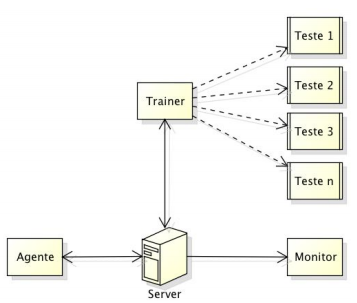
\includegraphics[scale=0.8]{figuras/trainer3d.png}
\caption{Arquitetura da ferramenta Trainer3D.} 
\label{fig:trainer3d}
\end{figure}
\FloatBarrier

Quando o Trainer3D é instanciado, ele gera uma comunicação com o servidor SimSpark através de um socket com protocolo TCP/IP que capta as 
mensagens do estado do agente, bola e campo. A partir da comunicação do trainer com o servidor, as mensagens que o servidor envia são 
quebradas em tokens que contém informações do ambiente que está sendo simulado e que são renderizadas pelo RoboViz.

Além de captar as mensagens do servidor, o trainer também possui a característica de mudar o estado do ambiente. Para mudar o estado do ambiente, 
mensagens específicas são enviadas ao servidor. Cada mensagem para alterar o estado de um objeto no ambiente deve conter um identificador que 
indica qual objeto deve ser atualizado.

As mensagens que o Trainer3D recebe possuem informações como posicionamento da bola e dos agentes que estão no campo. Com 
essas informações, é possível fazer uma análise de como o agente está atuando, se está caído, qual a velocidade média de deslocamento 
do agente, se a bola foi chutada, e outras informações.

Com o desenvolvimento da ferramenta, foi possível coletar os resultados dos testes realizados com os cenários pré-definidos de forma 
automatizada, sem a necessidade de interfer\^encia humana.

\section{Cenários de Teste}
\label{sec:cenarios}
O objetivo dos cenários de teste foi diversificar as situações em que o agente (ou robô) pudesse utilizar o modelo para encontrar
a melhor trajetória para realizar o seu objetivo, que no caso foi definido como efetuar um passe para um outro agente aliado. Um 
passe no futebol é fazer com que um agente $A$ chute a bola para um agente $B$, de modo que o agente $B$ possa receber a bola em 
uma posição estratégica.

Os cenários foram divididos em níveis de dificuldade. O nível de dificuldade foi definido como a quantidade de agentes oponentes, 
que são considerados obstáculos móveis que podem comprometer a realização do objetivo do agente que vai efetuar o passe da bola. Os 
níveis foram mapeados de acordo com a tabela \ref{tab:niveisDificuldade}.

\begin{table}[!htb]

\scalefont{0.8}

\centering

\caption{Nível A é considerado fácil, o B é considerado moderado, C é considerado difícil, e o D é considerado muito difícil.}

  \begin{tabular}{|c|c|}
    \hline
    Quantidade de oponentes & Nível de dificuldade \\ \hline
    2  & A \\ \hline
    3  & B \\ \hline
    4  & C \\ \hline
    4+ & D \\ \hline
  \end{tabular}

  \label{tab:niveisDificuldade}
\end{table}

Na figura \ref{fig:cenario}, são demonstradas as situações escolhidas para realizar os testes utilizando agentes oponentes que não se movem. 
Nestas situações, o objetivo foi verificar se o agente estava escolhendo a melhor trajetória para efetuar o passe e o 
executando corretamente.

\begin{figure}[!htb]
\centering
\scalefont{1.0}
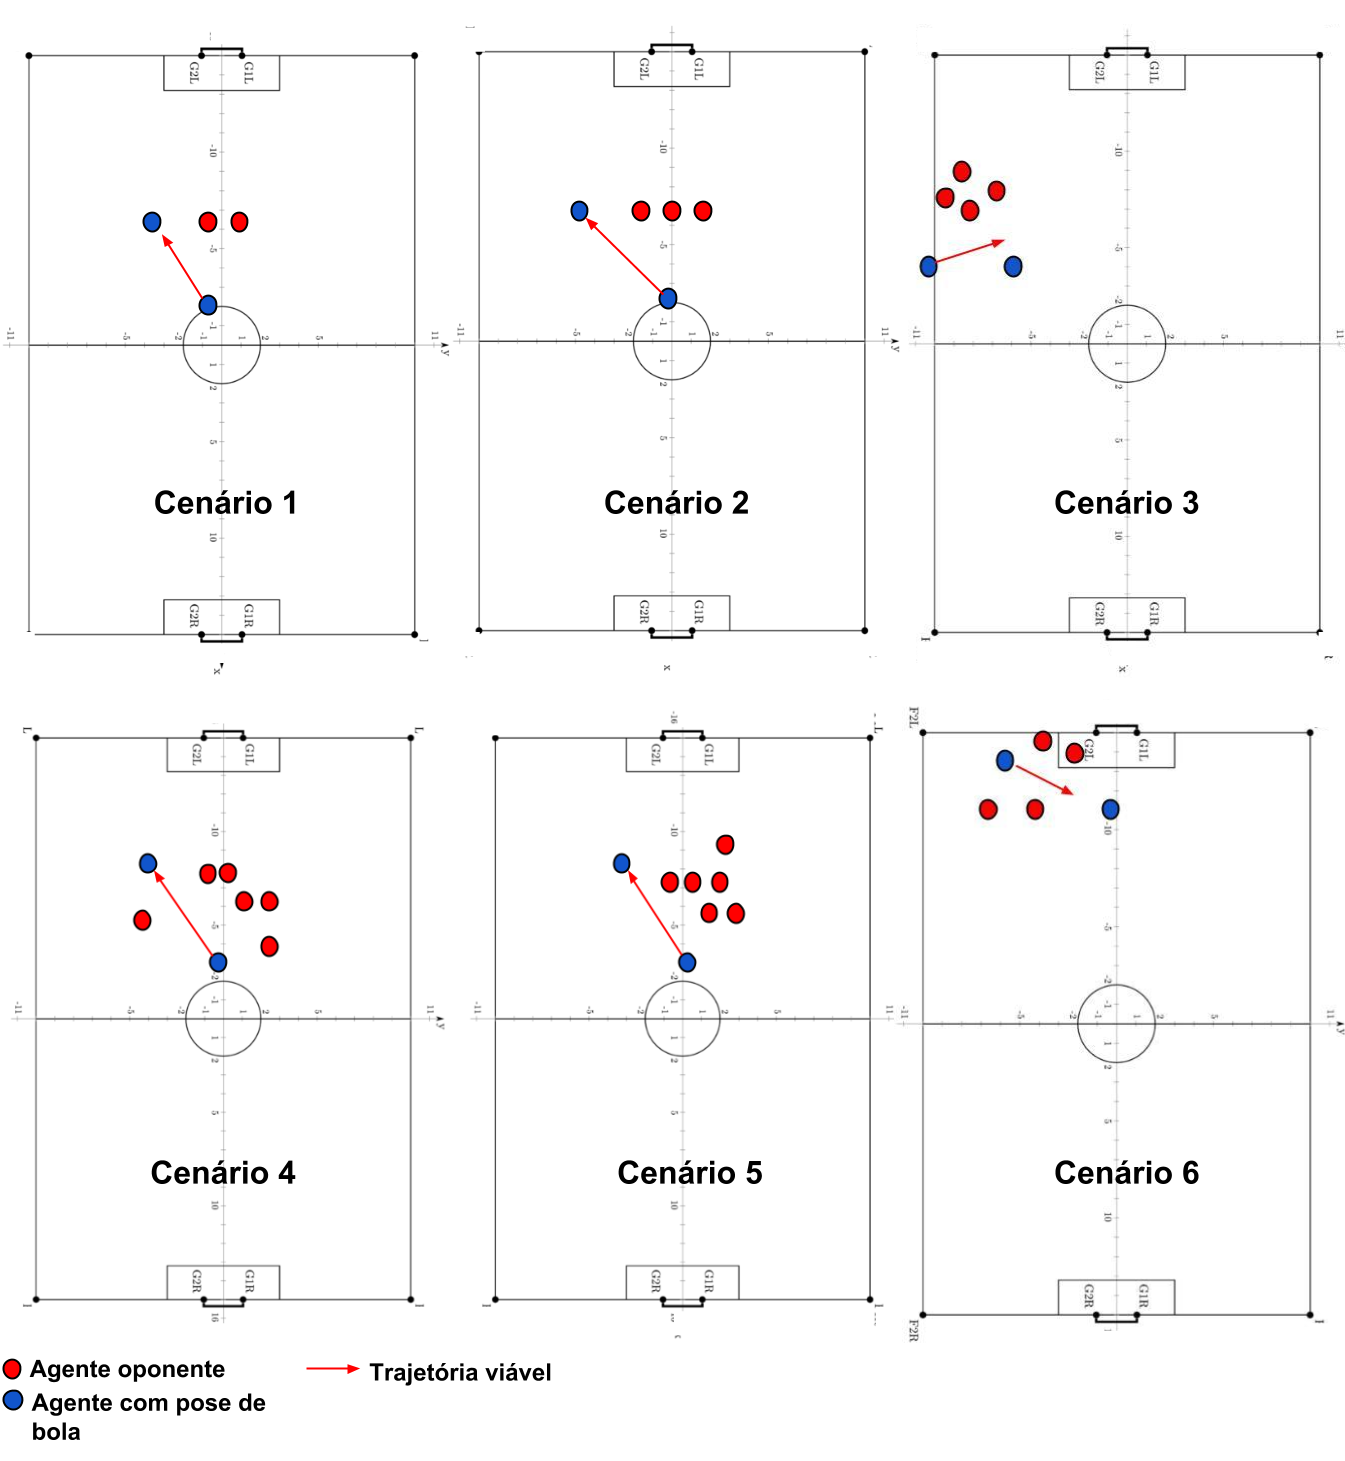
\includegraphics[scale=0.3]{figuras/Cenario.png}
\caption{Cenários de situações de um jogo real de futebol onde um agente tem a possibilidade de efetuar um passe para outro agente 
aliado em uma posição estratégica.} 
\label{fig:cenario}
\end{figure}
\FloatBarrier

\section{Métricas de Avaliação}
\label{sec:metricas}
Os indicadores escolhidos para validar o modelo proposto foram mapeados levando em consideração aspectos que não são 
influênciados por problemas que não estão dentro do contexto do problema em questão, que é o planejamento de trajetória em tempo 
real.

Para o primeiro processo de validação, foram definidas $5$ métricas:

\begin{enumerate}
    \item Quantidade total de passes
    \item Quantidade de passes corretos em kickin
    \item Quantidade de passes corretos em goal\_kik
    \item Quantidade de passes corretos em play\_on
    \item Quantidade de passes errados
\end{enumerate}

Para o segundo processo de validação, a métrica utilizada para validar o modelo foi a escolha da trajetória com base no 
cenário de teste executado.

Os testes executados que não estavam de acordo com a especificação da metodologia adotada, foram desconsiderados. O objetivo foi 
ter resultados bem definidos, que não foram afetados por outros problemas que ainda são lacunas a serem resolvidas em 
trabalhos posteriores.

\section{Resultados} 
\label{resultados}
O objetivo dessa seção é descrever os resultados obtidos no processo de validação através do ambiente real de jogo e de cenários 
pré-definidos. Todos os testes foram realizados utilizando o ambiente descrito na figura \ref{fig:arquiteturaAmbiente}. A análise 
dos resultados do primeiro processo de validação foi feita através do log gerado da partida pelo RoboViz, onde é possível reproduzir
todo o jogo, parando, voltando e adiantando quando necessário.

\subsection{Resultados de partidas utilizando cenário de jogo real}

Inicialmente foram realizadas $10$ partidas com alguns times da liga de simulação com duração de $10$ minutos cada partida. Os 
resultados preliminares demonstrados na tabela \ref{tab:resultado3}, mostraram que em mais de $40\%$ das tentativas de passe, 
onde o agente tinha condições favoráveis, o mesmo era cancelado por conta da demora para se posicionar e realizar o chute, e da
aproximação do agente adversário. Em alguns testes, quando o chute da bola alcançava uma dist\^ancia muito curta, os agentes 
oponentes conseguiam ter a pose de bola.

\begin{table}[H]

\scalefont{0.8}
\centering
\caption{Tabela com o resultados preliminares dos testes realizado com times da liga de simulação 3D}.

\begin{tabular}{|p{3cm}|c|c|c|c|c|}
    \hline
    Time & Apollo3D & UTAustinVilla & FCPortugal & ITAndroids \\ \hline
    Quantidade de passes	   				  & 57      & 54       & 35      & 105     \\ \hline
    Quantidade de passes corretos 				  & 8.77\%  & 18.52\%  & 31.43\% & 38.10\% \\ \hline
    Quantidade de passes que terminaram em gol 		  & 0.00\%  & 0.00\%   & 0.00\%  & 2.86\%  \\ \hline
    Quantidade de passes errados que terminaram em gol		  & 3.51\%  & 0.00\%   & 0.00\%  & 0.00\%  \\ \hline
    Quantidade de passes errados com pose de bola do adversário & 8.77\%  & 11.11\%  & 15.24\% & 15.24\% \\ \hline
    Quantidade de passes desistidos 				  & 78.95\% & 70.37\%  & 43.81\% & 43.81\% \\ \hline
  \end{tabular}

  \label{tab:resultado3}
\end{table}

Após a conclusão do projeto, foram realizadas $5$ partidas com duração de $10$ minutos para cada time. Os resultados obtidos 
no processo de validação final utilizando o cenário de jogo real demonstraram uma melhora significativa na quantidade de passes 
realizados com sucesso. Na tabela \ref{tab:resultado2} são demonstrados os resultados obtidos.  

\begin{table}[H]

\scalefont{0.8}
\centering
\caption{Tabela com o resultado dos testes realizado com times da liga de simulação 3D}.

  \begin{tabular}{|p{3cm}|c|c|c|c|c|}
    \hline
    Time & Mithras3d & UTAustinVilla & RoboCanes & Hfutengine \\ \hline
    Quantidade total de passes				& 15	 & 4   & 6  &  4\\ \hline       
    Quantidade de passes corretos em kickin	  	& 0      & 2   & 4  &  2\\ \hline
    Quantidade de passes corretos em goal\_kick 	& 0      & 2   & 2  &  	0\\ \hline
    Quantidade de passes corretos em play\_on 	  	& 15     & 0   & 0  &  	2\\ \hline
    Quantidade de passes errados	  		& 0	 & 0   & 0  &  	0\\ \hline
    
  \end{tabular}

  \label{tab:resultado2}
\end{table}

Os resultados obtidos demonstraram que em situações de bola parada, \textit{kickin}, \textit{goal\_kick}, 
onde o agente possui mais tempo para se posicionar e chutar a bola, os passes tiveram 100\% de acerto. Porém, em situações onde 
a bola está em jogo, \textit{play\_on}, sendo disputada por outros jogadores, ficou evidente que o principal fator responsável 
por permitir que o agente consiga efetuar mais passes é a velocidade com que o chute é executado. Contra o time Mithras3d, onde 
seus agentes possuia movimentação mais lenta, o agente conseguiu efetuar mais passes em modo \textit{play\_on}. Porém, contra o 
RoboCanes e UTAustinVilla, o agente não conseguiu efetuar passes em modo \textit{play\_on} devido a velocidade rápida da movimentação 
dos seus agentes. Ainda assim, nas situações de bola parada, os passes realizados permitiram ao BahiaRT obter vantagem estratégica.

\begin{table}[H]

\scalefont{0.8}
\centering
\caption{Tabela com o resultado das partidas realizadas no processo de validação}.

  \begin{tabular}{|p{3cm}|c|c|c|c|c|c|c|c|c|}
    \hline
    Time 		& Vitórias & Empates  & Derrotas & Gols Marcados & Gols Sofridos & Saldo de Gols \\ \hline
    Mithras3d	  	& 5        & 0   & 0  & 30  &  0 & 30  \\ \hline
    UTAustinVilla 	& 0        & 0   & 5  &  0  & 13 & -13 \\ \hline
    RoboCanes 	  	& 1        & 3   & 1  &  4  & 4  & 0 	\\ \hline
    Hfutengine	  	& 5	   & 0   & 0  & 22  & 0  & 22  \\ \hline
    
  \end{tabular}

  \label{tab:tabelajogos}
\end{table}

Na tabela \ref{tab:tabelajogos} são mostrados os resultados das partidas realizadas no processo de validação. Com o modelo de passe, 
o BahiaRT conseguiu obter maior aproveitamento, vencendo a maioria das partidas realizadas. Nos jogos realizados contra o time UTAustinVilla, 
o BahiaRT perdeu todas as partidas por conta do super chute realizado pelo time oponente. Tais gols não puderam ser evitados, pois foram realizados 
em situações de bola parada, nas laterais e no meio de campo. Já contra o Mithras3d e Hfutengine, o BahiaRT conseguiu obter maior aproveitamento de gols. 
Por último, o RoboCanes foi o time mais equilibrado, com forte marcação na defesa, dificultando as chances de passe e marcação de gols.

\subsection{Resultados utilizando cenários pré-definidos}
Os resultados obtidos no segundo processo de validação, onde foram realizados $20$ testes com situações pré-definidas 
demonstraram a eficácia do modelo desenvolvido em ambientes estáticos. Em todos os casos, o agente escolheu a melhor 
trajetória para efetuar o passe com base na segurança da trajetória e no posicionamento do agente aliado que recebeu o passe. 
Além disso, ficou evidente que independente do nível de dificuldade descrito na tabela \ref{tab:niveisDificuldade}, o 
agente consegue mapear e escolher a melhor trajetória.

Para demonstrar os resultados, foram plotados os pontos em que os agentes aliados e oponentes estavam posicionados e a
trajetória escolhida para realizar o passe utilizando o modelo desenvolvido. Foram plotadas \`as trajetórias na cor verde através 
de retas entre os pontos inicial e final, aliados com pontos em preto e oponentes em cor vermelha. Os resultados podem ser 
vistos nas figuras \ref{fig:cenario123} e \ref{fig:cenario456}.

%FIGURA COM OS RESULTADOS DOS AGENTES DUMMY

\begin{figure}[H]
\centering
\scalefont{1.0}
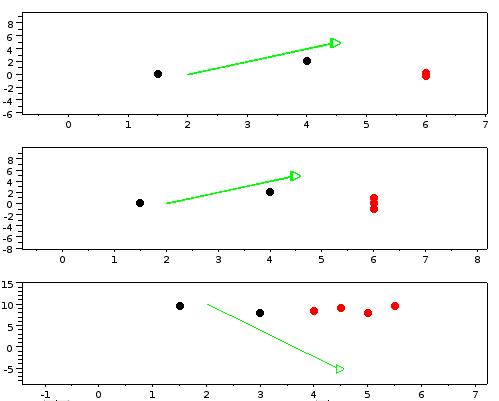
\includegraphics[scale=0.6]{figuras/cenario123.png}
\caption{Resultados dos testes realizados com agentes Dummy nos cenários pre-definidos.} 
\label{fig:cenario123}
\end{figure}
\FloatBarrier


\begin{figure}[H]
\centering
\scalefont{1.0}
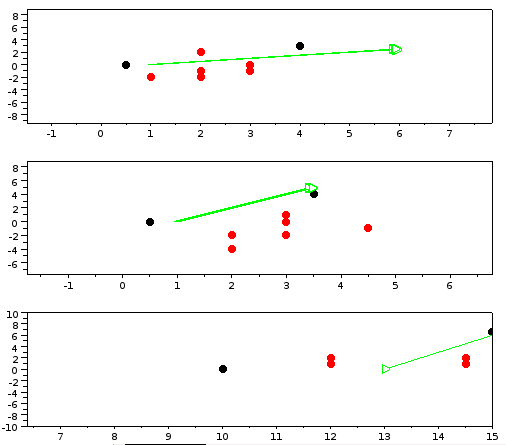
\includegraphics[scale=0.6]{figuras/cenario456.png}
\caption{Resultados dos testes realizados com agentes Dummy nos cenários pre-definidos.} 
\label{fig:cenario456}
\end{figure}
\FloatBarrier

    \chapter{Considerações Finais}
\label{chap:conclusao}

A construção de agentes bípedes aut\^onomos não é uma tarefa trivial. Além 
do comportamento de baixo nível que é representado por movimentos como andar, levantar os braços, chutar uma bola, 
é necessário desenvolver o comportamento de alto nível, onde o agente deve analisar as informações que possui, e 
a partir delas escolher a melhor ação a ser executada.

Este trabalho apresentou o desenvolvimento de um modelo para realizar o mapeamento e planejamento 
de trajetórias em tempo real para nagevação de agentes humanóides em ambiente simulado 3D. O objetivo 
do trabalho foi ter um modelo que possa ser utilizado no desenvolvimento de aplicações que 
requerem uma resposta rápida e ao mesmo tempo segura para guiar um agente através de um ambiente din\^amico. Como exemplo, podemos citar o resgate de pessoas em acidentes 
de desabamento, um agente inteligente deve ser capaz de se locomover no meio de destroços de concreto e buscar os 
melhores caminhos para chegar até a vítima de forma segura. Outra aplicação possível é a contrução de 
robôs de serviços que precisam navegar em ambientes onde prestarão serviços diversos aos humanos de forma 
segura e eficaz.

O modelo foi desenvolvido utilizando a linguagem C++, que é utilizada pelo time BahiaRT. Além disso, outras ferramentas 
como o Scilab, foi utilizada no desenvolvimento do algoritmo descrito na seção \ref{sec:calcvel}. 

Uma das contribuições trabalho é o Trainer3D. Esta ferramenta poderá ser utilizada por outros times da liga de simulação 3D 
para realizar testes, coletar indicadores de desempenho e automatizar o processo de otimização.

A validação do modelo se deu através do desenvolvimento de uma aplicação de passe. Esta aplicação foi escolhida 
para aumentar o nível estratégico do time BahiaRT, proporcionando jogadas que aumentem as chances de gol. Além disso, 
uma das principais motivações foi o principal campeonato mundial de futebol de rob\^os, a RoboCup.

Como trabalho futuro, a resolução dos problemas identificados no desenvolvimento da aplicação de passe se viu necessária. 
Estas influenciam diretamente a execução do passe no futebol robótico. Dentre os trabalhos, o desenvolvimento de um chute 
din\^amico é um trabalho imprescindível, pois engloba o rápido posicionamento para realizar um chute para qualquer direção.

    %
\section{Cronograma}
\begin{landscape}
    
    
    \begin{tabular}{|c|| c c c c c c c c c c c c c c c c c c c c|} 
    \hline 
    Atividades & \multicolumn{20}{c|}{Semanas} \\ 
	       & 1º & 2º & 3º & 4º & 5º & 6º & 7º & 8º & 9º & 10º & 11º & 12º & 13º & 14º & 15º & 16º & 17º & 18º & 19º & 20º\\ 
    \hline 
    \hline 
    
    Revisar a bibliografia		&X&X&X&X& & & & & & & & & & & & & & & &  \\%3
    básica pesquisada.			&X&X&X&X& & & & & & & & & & & & & & & &  \\
    \hline 
    Elaborar o modelo	 		& & & & &X&X&X&X& & & & & & & & & & & &  \\%5
					& & & & &X&X&X&X& & & & & & & & & & & &  \\
   \hline 
    Implementar o modelo 		& & & & & & & &X&X&X&X& & & & & & & & &  \\%5
    no agente				& & & & & & & &X&X&X&X& & & & & & & & &  \\
    \hline 
    Definir e realizar metodologia	& & & & & & & & & & &X&X&X& & & & & & &  \\%5
    de teste do modelo  		& & & & & & & & & & &X&X&X& & & & & & &  \\
    \hline 
    Realizar testes com o BahiaRT	& & & & & & & & & & & & & & &X&X& & & & \\%2
    \hline
    Realizar testes com outros times   & & & & & & & & & & & & & & & &X&X&X& & \\%2
    \hline 
    Testes finais			& & & & & & & & & & & & & & & & & &X&X&X \\ \\%2
    
\hline
    \end{tabular}
\label{tab:Cronograma}
\end{landscape}	
 
    \citeoption{abnt-etal-cite=10}

    \bibliography{referencias}

    % Apêndice e Anexos
    %\apendice
    %\chapter{Título do Apêndice A}
bla bla bla bla bla bla bla bla bla bla bla bla

bla bla bla bla bla bla bla bla bla bla bla bla

%%%%%%%%%%%%%%%%%%%%%%%%%%%%%%%%%%%%%%%%%%%%%%%%%%%%%%%%%%%%%%%%%%%%%%

\chapter{Título do Apêndice B}
bla bla bla bla bla bla bla bla bla bla bla bla

bla bla bla bla bla bla bla bla bla bla bla bla

    %\anexo
    %
\chapter{Título do Anexo A}
\vspace{-3cm}
bla bla bla bla bla bla bla bla bla bla bla bla

bla bla bla bla bla bla bla bla bla bla bla bla

%%%%%%%%%%%%%%%%%%%%%%%%%%%%%%%%%%%%%%%%%%%%%%%%%%%%%%%%%%%%%%%%%%%%%%

\chapter{Título do Anexo B}

bla bla bla bla bla bla bla bla bla bla bla bla

bla bla bla bla bla bla bla bla bla bla bla bla

%%%%%%%%%%%%%%%%%%%%%%%%%%%%%%%%%%%%%%%%%%%%%%%%%%%%%%%%%%%%%%%%%%%%%%

    
\end{document}